\section{Introduction}


\section{Wildfire Spread}

The foundation of ELMFIRE is the Rothermel model \cite{rothermelMathematicalModelPredicting1972, albiniEstimatingWildfireBehavior1976}, which estimates the head fire rate of spread in the direction of the wind and slope combined. An extensive and thorough guide has been compiled by Andrews \cite{andrewsRothermelSurfaceFire2018} covering all the aspects of the model, the input parameters, experimental background and corellations between values. For completeness, and consistency of units used in ELMFIRE, critical parts of the model will be repeated in this section. 

The Rothermel model, at a high level, outlines the rate of spread of a wildfire as an energy argument, specifically as the ratio of the energy produced by the fire front and the energy required for ignition. Rigorously, it is:

\begin{equation}
    R=\frac{I_R\xi(1+\phi_w+\phi_s)}{\rho_b\epsilon Q_{ig}}
\end{equation}

In general terms, the numerator is the propagating flux, and the denominator is the heat required to ignite the next parcel of fuel. Analytically:

\begin{itemize}
    \item $R$: Rate of Spread (ft/min): 1D velocity of the flaming front aligned with prevailing wind and slope.
    \item $I_R$: Reaction Intensity $(BTU/ft^2/min)$, energy released per unit area of fire front.
    \item $\xi$: Propagating Flux Ratio, fraction of released energy that reaches unburned fuel under no wind/slope.
    \item $\phi_w$: Wind Factor, dimensionless factor accounting for the effect of wind on the rate of spread. 
    \item $\phi_s$: Slope Factor, dimensionless factor accounting for the effect of slope on the rate of spread. 
    \item $\rho_b$ Fuel Bulk Density ($lb/ft^3$), oven-dry density of surface fuel.
    \item $\epsilon$: Effective Heating Number: Ratio of unburned fuel reaching ignition temperature before ignition.
    \item $Q_{ig}$: Heat of Preignition ($BTU/lb$): Energy required to ignite 1 lb of fuel. 
\end{itemize}

Of the above values, almost none are material values and they all need to be calculated through further equations and correlations. ELMFIRE makes no modifications to the Rothermel model as outlined in Andrews \cite{andrewsRothermelSurfaceFire2018}. Note that english units are used in the original model formulation, but metric equivalent equations have been developed.

From the above formulation of the Rothermel equation it may seem that the wind and slope must be aligned, and are then linearly added to the no-wind, no-slope rate of spread. Most of the times, the direction of maximum slope and the wind direction will not be matching, and need to go through vector addition instead. To do this, we can rewrite the Rothermel model as:

\begin{equation}
    R=V_{s,0}\alpha(1+ \| \vec{\phi_w}+\vec{\phi_s} \| ) =V_{s,0}\alpha(1+ \| \vec{\phi} \| )  
\end{equation}

where $V_{s,0}$ is the no-wind, no-slope rate of spread estimated by the Rothermel model, and $\alpha$ is a constant added by ELMFIRE to account for point source acceleration (only relevant in the early stages of the fire) such that $0 \leq \alpha \leq 1$. By assuming that the directional effects of wind and slope are independent, $\phi_x$ and $\phi_y$ (the $x$ and $y$ components of an “overall” $\vec{\phi}$) can be calculated with:

\[
\phi_{x} = \alpha(\phi_{w,x} + \phi_{s,x})
         = \alpha\!\left[\phi_{w} \sin(\theta_{w}-\pi) + 
                         \phi_{s} \sin(\theta_{a}-\pi)\right]
\]

\[
\phi_{y} = \alpha(\phi_{w,y} + \phi_{s,y})
         = \alpha\!\left[\phi_{w} \cos(\theta_{w}-\pi) + 
                         \phi_{s} \cos(\theta_{a}-\pi)\right]
\]

Then, by adding the constituents of the vector, 

\[
|\vec{\phi}| = \sqrt{\phi_{x}^{2} + \phi_{y}^{2}}
\]

Finally, the direction of maximum spread (the direction toward which the fire spreads most rapidly, i.e. the head fire direction) is calculated as:

\[
\theta_{DMS} =
\begin{cases}
\frac{\pi}{2} - \tan^{-1}\!\left(\dfrac{\phi_{y}}{\phi_{x}}\right),
    & \phi_{x} > 0 \;\text{and}\; \phi_{y} \ge 0 \\[1em]

\frac{3\pi}{2} - \tan^{-1}\!\left(\dfrac{\phi_{y}}{\phi_{x}}\right),
    & \phi_{x} < 0 \;\text{and}\; \phi_{y} \ge 0 \\[1em]

\frac{3\pi}{2} - \tan^{-1}\!\left(\dfrac{\phi_{y}}{\phi_{x}}\right),
    & \phi_{x} < 0 \;\text{and}\; \phi_{y} < 0 \\[1em]

\frac{\pi}{2} - \tan^{-1}\!\left(\dfrac{\phi_{y}}{\phi_{x}}\right),
    & \phi_{x} > 0 \;\text{and}\; \phi_{y} < 0
\end{cases}
\]

An effective midflame windspeed can then be calculated to represent the combined effect of wind and slope as one effective wind value. Effective mid-flame wind speed is calculated by solving Equation 47 from \cite{rothermelMathematicalModelPredicting1972} based on the 20ft wind speed and slope inputs, vector added to the parameter $\phi$:

\begin{equation}
U_{m,f,e} = 
\left(
\frac{\,|\phi|\,}{C \left( \frac{\beta}{\beta_{op}} \right)^{-E}}
\right)^{\frac{1}{B}}
\end{equation}

The parameters $C$, $\beta$, $\beta_{op}$, $E$, and $B$ are defined in \cite{rothermelMathematicalModelPredicting1972} and depend on the fuel model.

\subsection{The Canadian Fire Spread Model}

ELMFIRE can also use the Canadian FBP model to estimate maximum rate of spread. all other parts of ELMFIRE, such as the elliptical rate of spread breakdown and canopy fire effects, stay the same. The FBP system is a purely empirical set of models, derived from historic observations of natural and prescribed wildfires throughout Canada. Its development is well documented in a series of reports by the Canadian Forestry Service \cite{vanwagnerDevelopmentStructureCanadian1987, DevelopmentStructureCanadian1992, wottonUpdatesRevisions19922009, tymstraDevelopmentStructurePrometheus2010}. The main equations and workflow of the models will be repeated in this section, but no modifications are made in ELMFIRE.

The main equation for calculating the maximum rate of spread is shown below. The equations in the section below broadly apply to all fuel models, although some special cases apply for fuel models O1a, O1b (grass fuels), M1, M2, M3 and M4 (mixedwood stands).

\begin{equation}
    RSI = a(1-\exp(-b \times ISI))^{c}\times CF\times BE
\end{equation}

Where $a$, $b$ and $c$ are fuel model parameters, $ISI$ is the initial spread index, part of the FWI, $CF$ is the curing factor, only relevant for grass-type fuels, and $BE$ is the build-up effect, a function of the Build-Up Index (BUI). 

\[
BUI = \frac{0.8\times DMC\times DC}{DMC+1.4DC}
\]

$DMC$ and $DC$ are calculated using a starting value and an incoming weather stream, with no changes from the standard fire weather index calculations. 

$ISI$ is a function of wind and fuel moisture. Note that "wind" in this function represents effective wind, a vector combination of actual measured wind (at 10 m height) and wind-equivalent slope. 

\[
ISI = 0.208f(F)f(W)
\]

\[
f(F) = 91.9\,\exp(-0.1386\,M)
\left(1 + \frac{M^{5.31}}{4.93 \times 10^{7}}\right)
\]

\[
f(W) = 
\begin{cases}
\exp\!\left(0.05039\,\bar{U}\right),
& \text{if } 1.61\,U \le 40, \\[6pt]
12\left(1 - \exp\!\left(0.0818\,(\bar{U} - 28)\right)\right),
& \text{if } 1.61\,U > 40
\end{cases}
\]

Where M is the fine fuel moisture content (set as the 1h fuel moisture content in ELFMIRE, ranging from 0 to 1), $\bar{U}$ is the effective wind speed, and $U$ is the actual 10m wind speed in kph. The process of finding the effective wind speed requires finding the slope-only rate of spread and converting that value back into an equivalent wind speed. This is done by:

\begin{equation}
    RSF = RSZ \times SF
\end{equation}

\[
SF =
\begin{cases}
\exp\!\left( 3.533 \left[\tan\!\left(a\right)\right]^{1.2} \right),
& \text{if } a \le 63, \\[6pt]
10,
& \text{if } a > 63
\end{cases}
\]

\[
RSZ=a(1-\exp(-b \times ISI_0))^{c}\;,\;\;\; ISI_0=0.208f(F)
\]

Where $a$ is the slope in degrees. $RSF$ is then used in reverse to find the wind-based ISI for the given slope, yielding a slope-equicalent wind. Vector addition of the slope-equivalent wind and the actual wind then produce the effective wind $\bar{U}$. 

\subsection{Wind Scaling}

As might have been hinted at in the previous section, the wind factor in the Rothermel equation depends on the midflame windspeed, that is the wind at the height of the flames. Most weather stations and weather measurements in the world require wind be measured at some height above ground, to capture ``free wind velocity'' and avoid ground effects. In the US, that height is 20ft, while in other parts of the world it is 10m. 

ELMFIRE as standard expects wind inputs in mph and at 20ft height. Readings at 10m height are also acceptable, and are internally converted to 20ft readings by multiplying them by a constant 0.87. Then the wind needs to be scaled again to be brought down to midflame height. This requires the calculation of the wind adjustment factor, which is explained in depth in \cite{andrewsModelingWindAdjustment2012}. This final scaling depends on the flame length, which is assumed to be equal to the fuel bed depth. It also depends on the existence of canopy, as it would further reduce the midflame wind speed. For unsheldered surface fires (in the case of ELMFIRE, cases with canopy cover percentage of 0), the following conversion is used:

\[
U_{mf} = U_{20} \times WAF
\]

\begin{equation}
   WAF = \frac{1.83}{\ln\left(\frac{20+0.36H}{0.13H}\right)}
\end{equation}

For sheltered surface fires:

\begin{equation}
    WAF = \frac{0.555}{\sqrt{fH}\ln\left(\frac{20+0.36H}{0.13H}\right)}
\end{equation}

Where:

\begin{itemize}
    \item $H$: Fuel bed depth (ft)
    \item $f=\frac{CC}{100}\frac{\pi}{12}$
    \item $CC$: Canopy Cover (\%)
\end{itemize}

When the Canadian FBP system is used, and Fuel bed depth is not a parameter that the fuel model system stores, an alternative WAF calculation method is used based on \cite{scottNomographsEstimatingSurface2007}, using canopy cover ($CC$):

\[
WAF =
\begin{cases}
0.10 & \text{if } CC > 50 \\
0.15 & \text{if } 30 < CC \le 50 \\
0.20 & \text{if } 15 < CC \le 30 \\
0.25 & \text{if } 10 < CC \le 15 \\
0.30 & \text{if } 5 < CC \le 10 \\
0.50 & \text{if } CC \le 5
\end{cases}
\]

This midflame windspeed can then be used to calculate the wind adjustment factor. 

\subsection{Directional Rate of Spread}

The Rothermel model provides the head fire rate of spread; the spread rate at any angle from the head fire is needed for landscape spread calculations. ELMFIRE implements the elliptical wildfire propagation proposed by Anderson \cite{andersonPredictingWinddrivenWind1983} and later modified by Finney \cite{finneyFARSITEFireArea1994}. This theory suggests that wildfire spread from a point source can be described by an ellipse, following from experimental observation and a balance for ease of mathematical description. The equations describing the dimensions of the ellipse ultimately can be solved to find the rate of spread about any angle $\omega$ from the maximum spread direction. The dimensions of the ellipse are dictated by the following equation, describing the Length/Width ratio of the ellipse based on the effective midflame windspeed in mph $U_{mf,e}$:

\begin{equation}
    \frac{L}{W} = \min \left[ 
0.936\, e^{0.1147\, U_{mf,e}} 
+ 0.461\, e^{-0.0692\, U_{mf,e}} 
- 0.397,\; 8
\right]
\end{equation}

As in FARSITE, the maximum value of L/W is limited to 8 by default but in ELMFIRE this is a user-specifiable parameter. ELMFIRE computes this equation directly, compared to older versions of the code that used polynomial approximations.

The equations below show how the rate of spread is calculated, with $V_{DMS,\parallel}$ being the rate of spread at direction of maximum spread parallel to the ground, $V_{s0}$ being the backing rate of spread assumed equal to the no-wind/no-slope spread rate, and $\omega$ being the angle from the maximum spread direction.

\begin{align}
U^{*}_{y,\parallel} &= 
\frac{a^{2}\cos(\omega)}{\sqrt{a^{2}\cos^{2}(\omega) + b^{2}\sin^{2}(\omega)}} + c \\[1em]
U^{*}_{x,\parallel} &=
\frac{b^{2}\sin(\omega)}{\sqrt{a^{2}\cos^{2}(\omega) + b^{2}\sin^{2}(\omega)}} \\[1em]
a &= \frac{1}{2}\left( \left| V_{DMS,\parallel} \right| + V_{s0} \right) \\[0.5em]
b &= \frac{1}{2} \left| V_{DMS,\parallel} \right| + V_{s0} \frac{L}{W} \\[0.5em]
c &= \frac{1}{2}\left( \left| V_{DMS,\parallel} \right| - V_{s0} \right)
\end{align}

\subsection{Canopy Fires}
\label{math:canopy}
A review of canopy fire modelling systems can be found in \cite{scottComparisonCrownFire2006}. The one implemented in ELMFIRE is similar to that in Farsite \cite{finneyFARSITEFireArea1994, finneyFARSITEFireArea1998}. The criterion for a canopy fire starting is the critical fireline intensity of the surface fire, $I_0$,depends on the height of the crown base (CBH, m) and the canopy foliar moisture content (M, \%), following Van Wagner's model \cite{wagnerConditionsStartSpread1977} and the adjustments from Cruz et al \cite{cruzDevelopmentTestingModels2005}. It is calculated by:

\begin{equation*}
    I_0 = \left[0.010 CBH (460+25.9M)\right]^{3/2}
\end{equation*}

Then the ``intensity'' of the crown fire is dictated by another value, the critical minimum rate of spread for active canopy fire, $R_0$, calculated through the Crown Bulk Density, $kg m^{-3}$:

\begin{equation*}
    R_0 = 3.0/CBD
\end{equation*}

And the predicted rate of spread of the canopy fire, $R_{C,P}$ can be calculated using the CBD, 10m wind in kph (note the unit and reference height change), and $M_1$ being the 1-hour fuel moisture content of the surface fuel. Due to its direct dependence on wind, this model is not applicable for zero-wind conditions, which would only be encountered in idealized conditions. hence this case will be run similarly to the ``Windy'' case. 

\begin{equation*}
    R_{C,P} = 11.02\times U_{10}^{0.9}\times CBD^{0.19}\times \exp(-0.17\times M_1)
\end{equation*}

The combination of the two values can be used to determine if and what kind of crown fire occurs, depending on the surface fire fireline intensity $I_b$:

\begin{enumerate}
    \item Passive Crown Fire ($Ib \geq Io$ but $R_{C,P}/R_0<=1$)
    \item Active Crown Fire ($Ib \geq Io$, $R_{C,P}/R_0>1$)
    \item Independent Crown Fire ($Ib>Io$, $R_{C,P}/R_0>1$)
\end{enumerate}

Then, if the fire is determined to be a passive crown fire, its rate of spread will be adjusted to:

\begin{equation*}
    R_C=R_{C,P}\times \exp{\left(-CAC\right)}
\end{equation*}

For an active crown fire, the following equation is used, as long as the canopy cover of that point in the landscape exceeds the critical canopy cover (set by default as 0.39):

\begin{equation*}
    R_C=R_{C,P}
\end{equation*}

The calculated rate of spread of the canopy fire, whether passive or active, is then converted to an effective wind factor, to directly affect the calculated surface rate of spread. This way ELMFIRE can directly use the surface spread model to also include crown fire acceleration effects. The new effective wind factor $\phi_{w,e}$ is the maximum value between the Rothermel wind factor, $\phi_{w,R}$, and the Cruz canopy wind factor $\phi_{w,C}$, calculated by:

\begin{equation*}
    \phi_{w,C} = \frac{R_C}{R_{R,0}}-1
\end{equation*}

With ${R_{R,0}}$ being the no wind, no slope Rothermel predicted surface rate of spread. The calculation is then repeated to find the modified, surface-canopy coupled rate of spread. 

\subsection{Level Set Propagation}

At this stage the head rate of spread, the direction of primary spread, the rate of spread about any direction and canopy effects have been quantified. ELMFIRE can now use the level set method to spread the wildfire about a 2d landscape. The level set method is a common mathematical concept used to solve differential equations, find local maxima or minima, or solve for a specific variable, formulated in \cite{lautenbergerWildlandFireModeling2013}, building upon the work of \cite{rehmFirefrontPropagationUsing2009}. In this case, ELMFIRE restructures the problem of fire spread across a landscape as a differential equation, solving for time. The exact formulation is:

\[
\frac{\partial \phi}{\partial t}
+ U_x \frac{\partial \phi}{\partial x}
+ U_y \frac{\partial \phi}{\partial y}
= 0
\]

$\phi$ has no physical meaning except that the $\phi = 0$ isopleth (or level set) corresponds to the fire front. This provides a convenient way to track a curved surface, such as a fire front, on a regular grid. ELMFIRE integrates the governing PDE using a narrow-band formulation \cite{sethianFastMarchingLevel1996} with a second-order Runge--Kutta method and superbee flux limiters to prevent numerical oscillations.

In a previous step we had derived the values $U^{*}_{y,\parallel}$ and $U^{*}_{x,\parallel}$. Those are the y- and x-directions rate of spread about the rothermel-calculated main spread direction, parallel to the ground. To use them in the level set method, they first have to be realigned about the main coordinate grid, and then projected flat. As such, the orthogonal rate of spread components can be calculated by:

\[
U_{x,\parallel} = U^{*}_{y,\parallel}\,\sin(\theta_{DMS})
                 + U^{*}_{x,\parallel}\,\cos(\theta_{DMS})
\]

\[
U_{y,\parallel} = U^{*}_{y,\parallel}\,\cos(\theta_{DMS})
                 - U^{*}_{x,\parallel}\,\sin(\theta_{DMS})
\]

And then to correct for slope:

\[
\frac{U_{x}}{U_{x,\parallel}} 
= 1 - \left| \sin(\theta_{a}) \right|\,(1 - \cos(\gamma))
\]

\[
\frac{U_{y}}{U_{y,\parallel}} 
= 1 - \left| \cos(\theta_{a}) \right|\,(1 - \cos(\gamma))
\]

With $\theta_\alpha$ being the topographical aspect, and $\gamma$ being the topographical slope. This correction has the correct limiting behavior, firstly resulting in 1 in flat terrain. Now take the case of an east-facing slope ($\theta_a = \pi/2$). Since $\sin(\pi/2) = 1$, $U_x / U_{x,\parallel} = \cos(\gamma)$.
However, the $y$-direction spread rate is unaffected since $\cos(\pi/2) = 0$
and $U_y / U_{y,\parallel} = 1$.

The fire front can propagate only normal to itself. A key part of calculating the spread rate along the fire front is the normal vector to the $\phi$ field, representing the direction of spred of the fire front. This is shown graphically in Fig. \ref{fig:theta}. 

\[
\hat{n}
= \frac{1}{|\nabla \phi|}
\left(
\frac{\partial \phi}{\partial x}\,\hat{i}
+
\frac{\partial \phi}{\partial y}\,\hat{j}
\right)
= n_x \hat{i} + n_y \hat{j}
\]

\[
|\nabla \phi|
= \sqrt{
\left( \frac{\partial \phi}{\partial x} \right)^2
+
\left( \frac{\partial \phi}{\partial y} \right)^2
}
\]

Now we can define $\theta_n$ as the angle to which the $\phi$ field normal vector points about our reference grid system:

\[
\theta_n =
\begin{cases}
\frac{\pi}{2} - \tan^{-1}\!\left(\dfrac{n_y}{n_x}\right),
    & n_x \ge 0,\; n_y \ge 0 \\[1em]

\frac{3\pi}{2} - \tan^{-1}\!\left(\dfrac{n_y}{n_x}\right),
    & n_x \le 0,\; n_y \ge 0 \\[1em]

\frac{3\pi}{2} - \tan^{-1}\!\left(\dfrac{n_y}{n_x}\right),
    & n_x \le 0,\; n_y \le 0 \\[1em]

\frac{\pi}{2} - \tan^{-1}\!\left(\dfrac{|n_y|}{n_x}\right),
    & n_x \ge 0,\; n_y \le 0
\end{cases}
\]

\begin{figure}
    \centering
    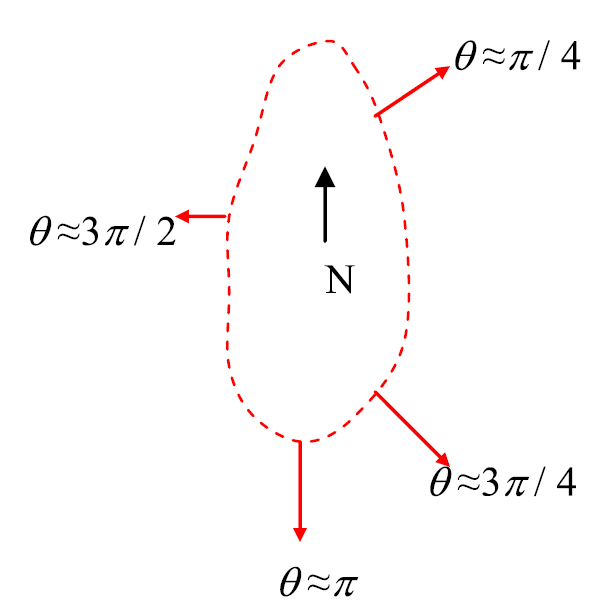
\includegraphics[width=0.55\linewidth]{figs/theta_explanation.png}
    \caption{Graphical illustration of $\theta$, the angle normal to fire front measured clockwise from North,at several locations along a sample fire perimeter.}
    \label{fig:theta}
\end{figure}


The steps in solving the ODE are given in good detail in Rehm and McDermott \cite{rehmFirefrontPropagationUsing2009}, and they will be repeated here based on their explanation. At any time step $t_n$ the gradient of $\phi$ can be calculated by central differentiation at each direction:

\[
\left( \frac{\delta \phi}{\delta x} \right)^{n}_{i,j}
= 
\frac{\phi^{n}_{i+1,j} - \phi^{n}_{i-1,j}}{2\,\Delta x},
\]

\[
\left( \frac{\delta \phi}{\delta y} \right)^{n}_{i,j}
=
\frac{\phi^{n}_{i,j+1} - \phi^{n}_{i,j-1}}{2\,\Delta y}.
\]

From these we can find the normal vector $\hat{n}$, and the angle $\theta_n$ of fire front spread. $U_x$ and $U_y$ can then be found by setting $\omega=\theta_{DMS}-\theta_n$. Before doing so, we set a flux limit to stabilise the ODE solver.

The central differentiation scheme used above can be reframed, using the $\phi$ values at the faces of the cell, in the example below the east and west face, instead of the centers of the adjacent cells:

\[
\frac{\delta \phi}{\delta x} = \frac{\phi_{east}-\phi_{west}}{\Delta x}
\]

We then define the local data ratio:

\[
r=\frac{\phi_{i+1,j} - \phi_{i,j}}{\phi_{i,j}-\phi_{i-1,j}}
\]

And the flux limiter function (Superbee):

\[
B(r) = max[0, min(2r,1),min(r,2)]
\]

The flux limiter can then be applied directly to the face values, such as:

\[
\phi_{east} = \phi_{i,j}+\frac{1}{2}B(\phi_{i+1,j}-\phi_{i,j})
\]

The rest of the face $\phi$ values can be computed similarly, based on the cell center $\phi$ values, and the original gradients of the ODE can be solved once again. 

To integrate the ODE through time, the second order RK scheme is used. The time step $\Delta t$ is controlled by the CFL criterion, set as standard as 0.2 but modifiable by the user. The mathematical formulation used in ELMFIRE is given below:

\begin{align}
\phi^{*} 
&= \phi^{t}
   - \Delta t \left(
        U_{x}^{t} \frac{\phi^{t}_{\text{east}} - \phi^{t}_{\text{west}}}{\Delta x}
      + U_{y}^{t} \frac{\phi^{t}_{\text{north}} - \phi^{t}_{\text{south}}}{\Delta y}
     \right)
\tag{10a}
\\[1em]
\phi^{t+\Delta t}
&= \tfrac{1}{2}\phi^{t}
   + \tfrac{1}{2}\left(
        \phi^{*}
        - \Delta t \left(
              U_{x}^{*} \frac{\phi^{*}_{\text{east}} - \phi^{*}_{\text{west}}}{\Delta x}
            + U_{y}^{*} \frac{\phi^{*}_{\text{north}} - \phi^{*}_{\text{south}}}{\Delta y}
        \right)
     \right)
\tag{10b}
\end{align}

And thus, each time step a new $\phi$ is calculated and the fire front is allowed to progress. For the first time step, ignition is dictated by the points where $\phi=1$.

\subsection{Acceleration}

The Rothermel model described above provides the equilibrium rate of surface fire spread, but in reality this equilibrium rate of spread is not achieved instantaneously \cite{finneyFARSITEFireArea1998, lautenbergerWildlandFireModeling2013}. Consequently, for initial ignition locations and spot fires that form during a simulation, the rate of spread increases from zero to the equilibrium spread rate as follows:

\[
\frac{R_{ac}}{R}
= 1 - \exp\!\left( -\,\frac{t - t_{\mathrm{ign}}}{\tau_{\mathrm{accel}}} \right)
\]

where $T_{ign}$ is the time (s) that a point is ignited (by the initial conditions or by a spot fire, and $\tau_{\mathrm{accel}}$ is a user specified acceleration time constant (s), usually on the order of 600.

\section{Spotting}

The process of a spot fire being created (generation, transport, ignition) can be broken up to its constituent processes, and each one can be studied separately. Much of the firebrand model in ELMFIRE is taken from the thesis of Yiren Qin from the University of Maryland \cite{qinPhysicsBasedEulerianFramework2025}, and will in large parts be reproduced below for completeness.

\subsection{Generation}

In ELMFIRE, the generation of firebrands is primarily controlled by two parameters: the \textbf{generation duration} ($t_g$) and the \textbf{generation rate} ($N$) of each computational cell. The firebrand generation duration is defined as the total time a cell is permitted to produce firebrands following its ignition. Ignition occurs when the local value of the level-set variable $\phi$ becomes less than or equal to 0. The generation rate $N$ represents the total number of firebrands produced by a computational cell during a single level-set equation solver time step ($\Delta t$). Users may specify an arbitrary rate, use physics-based estimations derived from literature correlations, or apply customized empirical parameters.

Three distinct approaches are available in ELMFIRE to define the generation rate:
\begin{itemize}
    \item \textbf{Mode A}: $N$ is randomly sampled from a bounded uniform distribution.
    \item \textbf{Mode B}: A constant generation rate is prescribed based on the number of firebrands per unit area per second.
    \item \textbf{Mode C}: A constant generation rate is prescribed based on the number of firebrands per megawatt of Heat Release Rate (HRR) per second (pcs/MW/s). In this mode, the generation rate $N$ correlates linearly with the local HRR.
\end{itemize}

Modes B and C are components of the UMD spotting model.

\textbf{Mode A: Stochastic Sampling}

For Mode A, the upper ($N_M$) and lower ($N_m$) bounds of the generation rate are prescribed. Upon cell ignition, $N$ is sampled from the uniform distribution $\text{Unif}[N_m, N_M]$, and the corresponding number of firebrands is generated during that time step. In this mode, firebrands are generated only once; thus, the effective generation duration is $t_g = \Delta t$.

\textbf{Mode B: Area-Based Generation}

Mode B defines the ember generation rate using a factor $G_t$, representing the number of firebrands per square meter per second ($\text{pcs/m}^2/\text{s}$). The generation rate is calculated as:
\[
N = G_t A_c \min(\Delta t, t_g - t_e)
\]
where $A_c$ is the cell area ($A_c = c^2$, where $c$ is the cell size), $\Delta t$ is the level-set solver time step, and $t_e$ is the elapsed time since the cell began emitting firebrands. The term $(t_g - t_e)$ represents the remaining generation window. This formulation ensures that the total number of generated firebrands remains consistent at $(t_g \times A_c \times G_t)$, independent of fluctuations in $\Delta t$ during the simulation.

\textbf{Mode C: HRR-Based Generation}

Mode C normalizes the generation rate by fire power using a factor $G$ ($\text{pcs/MW/s}$). The generation rate is defined as:
\[
N = \text{HRR} \times G \times \min(\Delta t, t_g - t_e)
\]
where $\text{HRR}$ is the heat release rate of the source cell in MW. Empirical values for $G$ are derived from literature, typically 33.3~pcs/MW/s for vegetative fuels and 10~pcs/MW/s for structural fuels. These values should be used with caution but can be modified by the user if site-specific data is available. 

For vegetative fuels, the HRR is estimated via fireline intensity and cell size ($\text{HRR} = I_f \times c$). For structural fuels, WUI surface fire models utilize a prescribed design fire curve based on HRR per unit area (HRRPUA); in this case, the local HRR is calculated as $\text{HRRPUA} \times A_c$.

\textbf{Computational Implementation}

When using Mode B or C, the resulting firebrand count $N$ is divided by an \textbf{ember sampling factor} (defaulting to 1) to manage computational load. Because the Lagrangian transport approach requires $N$ to be an integer, non-integer values are processed using \textbf{stochastic rounding}. The value is rounded to the nearest higher or lower integer with a rounding probability equal to its decimal component. For example, if $N = 1.6~\text{pcs}/\Delta t$ and the cell is expected to emit firebrands for 100 steps ($t_g = 100\Delta t$), we expect 60 steps to emit 2 firebrands and 40 steps to emit 1 firebrand. This approach ensures that the total number of generated firebrands converges to the expected value $(N \times t_g / \Delta t)$ when $\Delta t \ll t_g$. Consequently, a sufficiently small time step is recommended to achieve convergence when running the Lagrangian transport scheme.

\subsection{Transport}
\label{firebrand_transport}

ELMFIRE provides two primary approaches for modeling firebrand transport: a Lagrangian scheme and an Eulerian scheme. In both approaches, firebrands are assigned travel distances based on prescribed probability distributions.

In the Lagrangian scheme, the spotting distance is explicitly sampled for each firebrand from a specified probabilistic distribution. In contrast, in the Eulerian scheme, the probabilistic distribution is interpreted as a deposition distribution over the landscape. In this context, the distribution represents the spatial number density of firebrands after all firebrands emitted from a source under given conditions have landed.

Three types of probabilistic (or density) distributions are available in ELMFIRE:
(i) a user-defined uniform distribution,
(ii) a user-defined lognormal distribution, and
(iii) physics-based lognormal distributions parameterized following Sardoy et al.~\cite{sardoyNumericalStudyGroundlevel2008} and Himoto et al.~\cite{himotoTransportDiskshapedFirebrands2005}.

All three distributions are available in the Lagrangian scheme, whereas only the physics-based lognormal distributions are used in the Eulerian scheme. The following sections describe the formulation and sampling procedures used in the Lagrangian scheme.

\textbf{Uniform Distribution}

For the uniform distribution, the spotting distance is sampled within a prescribed range defined by minimum and maximum values. A random number is drawn from a uniform distribution over this interval, and the spotting distance is assigned accordingly.

\textbf{User-Defined Lognormal Distribution}
\label{math_lognormal}

The spotting distance $X$ is assumed to follow a lognormal distribution:

\[
pdf(X) = \frac{1}{X \, \sigma_x \sqrt{2\pi}} 
\exp\!\left[-\frac{(\ln X - \mu_x)^2}{2\sigma_x^2}\right].
\]

The parameters $\mu_x$ and $\sigma_x$ are related to the physical mean spotting distance ($\text{MSD}$) and its standard deviation ($v$) as:

\[
\mu_x = \ln\!\left(\frac{\text{MSD}^{2}}{\sqrt{\text{MSD}\cdot v + \text{MSD}^{2}}}\right),
\]

\[
\sigma_x = \sqrt{\ln\!\left(1 + \frac{\text{MSD}\cdot v}{\text{MSD}^{2}}\right)}.
\]

The mean spotting distance is further parameterized as:

\[
\text{MSD} = \overline{x} \, I_b^{a} U_{20}^{b}.
\]

Here, $\overline{x}$, $v$, $a$, and $b$ are empirical parameters that control the shape of the distribution. By default, $a = 0.5$ and $b = 0.9$, while $\overline{x}$ and $v$ are case-dependent.

In ELMFIRE, these parameters are specified in the \code{\&SPOTTING} namelist as follows: $\overline{x}$ corresponds to \code{MEAN_SPOTTING_DIST}, $v$ to \code{NORMALIZED_SPOTTING_DIST_VARIANCE}, $a$ to \code{SPOT_FLIN_EXP}, and $b$ to \code{SPOT_WS_EXP}.

Sampling is performed using inverse transform sampling. A random number $R_0 \sim \text{Unif}[0,1]$ is generated, and the spotting distance is computed as:

\[
X = \exp\left(\mu_x + \sqrt{2}\sigma_x \, \operatorname{erf}^{-1}(2R_0 - 1)\right).
\]

The right-hand side of the equation corresponds to the inverse of the cumulative distribution function (CDF) associated with the given probability density function (PDF). In ELMFIRE, $\operatorname{erf}^{-1}$ is evaluated using a sixth-order polynomial approximation for small arguments and a Winitzki analytical approximation for large arguments, providing a balance between accuracy and computational efficiency.

\subsubsection*{Physics-Based Lognormal Distribution}

For physics-based models, the downwind spotting distance $X$ follows:

\[
pdf(X) = \frac{1}{X \, \sigma_x \sqrt{2\pi}} 
\exp\!\left[-\frac{(\ln X - \mu_x)^2}{2\sigma_x^2}\right],
\]

where $\mu_x$ and $\sigma_x$ are determined from physical considerations.

\subsubsection*{Wildland Fuels}

For wildland fuels, the parameters follow Sardoy et al.~\cite{sardoyNumericalStudyGroundlevel2008}. The Froude number is defined as:

\[
Fr = \frac{U_{10}}{\sqrt{g L_c}}, 
\qquad 
L_c = \left(\frac{1000 \, I_b}{\rho_\infty c_{p,g} T_\infty \sqrt{g}}\right)^{2/3}.
\]

The lognormal parameters are:

For $Fr \le 1$:
\[
\mu_x = 1.47 \, I_b^{0.54} U_{10}^{-0.55} + 1.14,
\quad
\sigma_x = 0.86 \, I_b^{-0.21} U_{10}^{0.44} + 0.19.
\]

For $Fr > 1$:
\[
\mu_x = 1.32 \, I_b^{0.26} U_{10}^{0.11} - 0.02,
\quad
\sigma_x = 4.95 \, I_b^{-0.01} U_{10}^{-0.02} - 3.48.
\]

\subsubsection*{Urban/Structural Fuels}

For urban and structural fuels, the formulation of Himoto et al.~\cite{himotoTransportDiskshapedFirebrands2005} is used.

A characteristic length scale $L_c$ represents the building size (default $L_c = 10~\mathrm{m}$). The heat release rate is estimated as:

\[
Q = I_b \, L_c \times 1000.
\]

A dimensionless parameter $B^*$ is defined as:

\[
B^* = \frac{U_{10}}{\sqrt{g L_c}} 
\left(\frac{\rho_p}{\rho_\infty}\right)^{-3/4}
\left(\frac{D_p}{L_c}\right)^{-3/4}
\left(\frac{Q}{\rho_\infty c_{p,g} T_\infty \sqrt{g} \, L_c^{5/2}}\right)^{1/2}.
\]

The mean and standard deviation in physical space are:

\[
\mu_x^* = 0.47 \, B^{*\,2/3} \, L_c,
\quad
\sigma_x^* = 0.88 \, B^{*\,1/3} \, L_c.
\]

These are converted to lognormal parameters:

\[
\mu_x = \ln\!\left(\frac{\mu_x^*}{\sqrt{\left(\frac{\sigma_x^*}{\mu_x^*}\right)^2 + 1}}\right),
\quad
\sigma_x = \sqrt{\ln\!\left(1 + \left(\frac{\sigma_x^*}{\mu_x^*}\right)^2\right)}.
\]

To ensure numerical robustness when using physics-based lognormal distributions, the probability density function (PDF) is truncated over the interval $[0,\, X_{1 - P_{\text{EPS}}}]$, corresponding to the $(1 - P_{\text{EPS}})$ percentile:

\[
X_M = \exp\left(\mu_x + \sqrt{2}\sigma_x \, \operatorname{erf}^{-1}(2P_{\text{EPS}} - 1)\right).
\]

The truncation limit is aligned with the grid spacing $\Delta x$:

\[
X_M^* = \Delta x \left\lceil \frac{X_M}{\Delta x} \right\rceil.
\]

The truncated PDF is subsequently renormalized to ensure that its integral over the truncated domain equals unity:

\[
pdf^*(X) = \frac{pdf(X)}{\int_0^{X_M^*} pdf(X)\, dX}.
\]

Sampling is performed by mapping a uniform random variable to the truncated CDF:

\[
R_0^* = R_0 (S_H - S_L) + S_L,
\]

with

\[
S_L = \tfrac{1}{2}\left[1 + \operatorname{erf}\!\left(\frac{\ln(10^{-6}) - \mu_x}{\sqrt{2}\sigma_x}\right)\right],
\]

\[
S_H = \tfrac{1}{2}\left[1 + \operatorname{erf}\!\left(\frac{\ln(X_M + 0.5\Delta x) - \mu_x}{\sqrt{2}\sigma_x}\right)\right].
\]

The final sampled spotting distance is:

\[
X = \exp\left(\mu_x + \sqrt{2}\sigma_x \, \operatorname{erf}^{-1}(2R_0^* - 1)\right).
\]

The procedures described above provide the scalar distance that firebrands travel. The actual trajectory of the firebrands is then determined based on the input wind field. The treatment of particle accumulation and subsequent ignition during transport depends on whether a Lagrangian or Eulerian approach is used.

In the Lagrangian approach, firebrands are tracked individually and accumulate discretely at their landing locations. In the Eulerian approach, the probabilistic distribution is interpreted as a spatial deposition field, and firebrand number fluxes are distributed continuously along the transport trajectory. The details of each approach are described below.

\subsubsection{Lagrangian Model}

The Lagrangian model computes a unique, probabilistic landing location for each firebrand, or for each particle representing a group of firebrands defined by \texttt{EMBER\_SAMPLING\_FACTOR}, generated from a burning cell. The downwind displacement is determined by the wind velocity field and the sampled spotting distance from the distributions described previously.

After the spotting distance is sampled, the particle trajectory is integrated using a first-order Forward Euler scheme. Firebrands are assumed to be massless and therefore travel at the local wind speed. The particle position is updated as:

\[
\vec{X}_t = \vec{X}_{t-1} + \left(\vec{U}_{20} + \vec{\varepsilon}\right)\Delta t,
\]

where $\vec{X}_t = (x,y)$ denotes the particle position at time $t$, $\vec{U}_{20} = (U_{x,20},\, U_{y,20})$ is the 20-ft wind velocity vector, and $U_{x,20}$ and $U_{y,20}$ are its components in the $x$ and $y$ directions, respectively. The term $\vec{\varepsilon}$ represents a stochastic perturbation to the wind direction.

The integration time step $\Delta t$ is independent of the time step used in the level-set solver and is defined as:

\[
\Delta t = \min\!\left( \frac{0.5 \, \Delta x}{\max(\|\vec{U}_{20}\|,\, 0.01)}, \, 5.0 \right),
\]

which corresponds to a Courant--Friedrichs--Lewy (CFL) condition of 0.5 based on the 20-ft wind speed. The magnitude of the two-dimensional wind velocity vector is given by:

\[
\|\vec{U}_{20}\| = \sqrt{U_{x,20}^2 + U_{y,20}^2}.
\]

The trajectory is integrated until the accumulated travel distance reaches or exceeds the sampled spotting distance.

The perturbation term $\vec{\varepsilon}$ introduces a randomized angular deviation to account for turbulent fluctuations in the ambient wind. A fluctuation is sampled uniformly between $-4^\circ$ and $4^\circ$ for each particle and is applied consistently throughout the trajectory integration.

For example, if the sampled fluctuation is $1^\circ$, then at every time step (with interval $\Delta t$), the particle trajectory is deviated by $1^\circ$ from the local wind direction. This constant angular offset is maintained over the entire trajectory, representing a persistent turbulent effect.

For the UMD spotting model, an additional crosswind dispersion is incorporated. The crosswind displacement is modeled independently using a normal distribution centered on the downwind trajectory:

\[
pdf_y(Y) = \frac{1}{\sigma_y \sqrt{2\pi}} 
\exp\!\left[-\frac{1}{2}\left(\frac{Y - \mu_y}{\sigma_y}\right)^2\right],
\]

\[
\mu_y = 0, 
\qquad 
\sigma_y = 0.92 \, L_c,
\]

where $L_c$ is the characteristic length scale defined previously.

This dispersion is applied after the particle has reached its downwind travel distance. For example, if a particle terminates at $(x_{\mathrm{end}}, y_{\mathrm{end}})$ based on the trajectory integration, it is subsequently displaced in the direction normal to the trajectory. An offset distance is sampled from the normal distribution, and the particle is reassigned to the corresponding grid cell at that offset location.

The sampling is again performed using the inverse transform sampling method. A random number $R_0$ is first drawn from the unit uniform distribution $\text{Unif}[0,1]$. The crosswind displacement is then computed as:

\[
Y = \sqrt{2}\,\sigma_y \,\text{erf}^{-1}(2R_0 - 1) + \mu_y.
\]

At the end of the transport process, the number of firebrands deposited in each grid cell is accumulated and subsequently used in the ignition step.

\subsubsection{Eulerian Model}

The Eulerian model treats firebrand transport as a continuous, spatially distributed process, rather than tracking individual particles. Instead of assigning a discrete landing location to each firebrand, the model computes the evolution of a firebrand number density field, representing the expected deposition of firebrands over the computational domain. This formulation is consistent with the physics-based Eulerian framework developed by Qin et al.~\cite{qinPhysicsBasedEulerianFramework2025}.

In this approach, the downwind firebrand number distribution is described using the physics-based lognormal distribution introduced in the previous section, while the crosswind distribution is modeled independently using a normal distribution centered on the mean trajectory, consistent with the crosswind dispersion applied in the UMD spotting model in the Lagrangian scheme. The corresponding parameters $\mu_x$, $\sigma_x$, and $\sigma_y$ are determined from the fireline intensity and wind conditions, as described above.

Note that the crosswind distribution is truncated symmetrically such that the retained domain accounts for approximately 99\% (by default) of the original probability density function (PDF). The truncation bounds are further adjusted to align with the nearest grid boundaries to ensure numerical robustness of the scheme. This procedure defines a one-sided maximum crosswind distance, $Y_M^*$, measured normal to the firebrand trajectory.

To update the firebrand number distribution, the maximum transport distances in the downwind and crosswind directions, denoted as $X_M^*$ and $Y_M^*$, are first evaluated based on the truncated distributions. This treatment ensures that the required integrals are performed over a finite domain, thereby limiting the computational cost associated with firebrand transport while maintaining a negligible loss of the long-range tail of the distribution.

A tracer representing the transport path is then integrated over time using the same forward Euler scheme adopted in the Lagrangian model, with the total trajectory length equal to $X_M^*$. The time step is defined by a CFL condition:

\[
\mathrm{CFL} = \frac{\|\vec{U}_{20}\| \, \Delta t}{\Delta x} = 1.
\]

With this fixed time step, the tracer advances exactly one computational grid cell at each time step.

Based on this formulation, at the $k$-th time step following emission, the tracer originating from a source travels from $X_{k-1}$ to $X_k$, corresponding to cell $k$. Firebrands are then distributed within this cell and across neighboring cells in the crosswind direction according to the prescribed probability distributions. The number of firebrands allocated is proportional to the joint probability of deposition over the corresponding spatial intervals.

Consider a cell $l$ located in the crosswind direction, bounded by the interval $[Y_{k-1}, Y_k]$ relative to the trajectory. The probability of a firebrand landing in cell $l$ is given by:

\[
Pr_l = \left( \int_{X_{k-1}}^{X_k} pdf^*(x)\, \mathrm{d}x \right)
       \left( \int_{Y_{k-1}}^{Y_k} pdf_y^*(y)\, \mathrm{d}y \right).
\]

Similarly, for the central cell $k$ along the trajectory, the landing probability is:

\[
Pr_k = \left( \int_{X_{k-1}}^{X_k} pdf^*(x)\, \mathrm{d}x \right)
       \left( \int_{-0.5\Delta x}^{0.5\Delta x} pdf_y^*(y)\, \mathrm{d}y \right).
\]

Assuming that the emission source releases $N$ firebrands during the level-set solver time interval $\Delta t_l$ at time $t_0$, the number of firebrands allocated to cells $k$ and $l$ at time $(t_0 + k\times \Delta t)$ is given by $(N \times Pr_k)$ and $(N \times Pr_l)$, respectively. Note that $\Delta t_l$ is distinct from the time step $\Delta t$ used for tracer trajectory integration.

This deposition process is applied to all cells along the trajectory within the downwind range $[0,\, X_M^*]$, and across all crosswind cells within the range $[-Y_M^*,\, Y_M^*]$ normal to the trajectory, resulting in a spatial distribution of accumulated firebrands. The temporal evolution of this deposition field implicitly captures the arrival time distribution of firebrands, which is subsequently utilized in the ignition model.

\subsection{Ignition}

In ELMFIRE, ignition of target fuels by firebrands is modeled using two approaches: (1) a probabilistic method and (2) a physics-based method. The probabilistic approach is only compatible with the Lagrangian transport scheme, whereas the physics-based approach can be applied to both Lagrangian and Eulerian schemes, provided that the local evolution of the total firebrand number is properly accounted for.

\textbf{Probabilitic ignition model}

In the Lagrangian transport scheme, each deposited particle—either an individual firebrand or a particle representing a group of firebrands—is assigned an ignition probability $P_i$ upon landing.

The ignition process is modeled using stochastic sampling. Specifically, when a particle reaches its destination, a random number $R_0$ is drawn from a unit uniform distribution, $R_0 \sim \text{Unif}[0,1]$, and compared with $P_i$. If $R_0 \le P_i$, the target cell is considered ignited and the level-set variable is set to $\phi = -1$. Otherwise, the particle is discarded for ignition purposes, and subsequent ignition of the same cell depends on the arrival of other particles.

Under the default configuration, all deposited firebrands lead to ignition, corresponding to $P_i = 1$.

In addition, a final spatial consistency check is applied in the default ELMFIRE ignition model within the Lagrangian scheme. A $7 \times 7$ kernel centered at the landing location is evaluated. If any cell within this kernel is already part of the fire front (i.e., $\phi < 0$), the firebrand is considered sufficiently close to the existing fire, and no additional spot fire is initiated.

\textbf{Physics-based ignition model}

In ELMFIRE, a physics-based ignition model is available in addition to the probabilistic approach described above. Ignition of a target cell receiving firebrands is implemented by setting the level-set variable $\phi$ to $-1$ at time $t = \mathrm{TOA} + t_{\text{ignition}}$, where $\mathrm{TOA}$ denotes the time of arrival of the first firebrand, and $t_{\text{ignition}}$ is the time required for the fire to reach a sufficiently developed state.

The ignition process is modeled as two consecutive stages: (i) the formation of a local small flame (associated with smoldering-to-flaming transition), and (ii) the transition from a small flame to a fully developed fire. Accordingly, the total ignition time is defined as:
\begin{equation}\label{eq:t_ign_def}
t_{\text{ignition}} = t_{\text{ign,small}} + t_{\text{ign,large}},
\end{equation}
where $t_{\text{ign,small}}$ represents the time required to establish a small flame, and $t_{\text{ign,large}}$ represents the subsequent transition time to a fully developed fire.

\paragraph{Modeling of $t_{\text{ign,small}}$}

In the present formulation, $t_{\text{ign,small}}$ is treated as a random variable determined from a probabilistic ignition model. Let $P_{\text{ign,small}}$ denote the probability that firebrands ignite a small flame on a flammable substrate within a specified duration $\tau_{\text{ign,small}}$:
\begin{equation}\label{eq:p_ign_small_def}
P_{\text{ign,small}} = \mathrm{Probability}\!\left(t_{\text{ign,small}} \le \tau_{\text{ign,small}}\right).
\end{equation}

Models for $P_{\text{ign,small}}$ and $\tau_{\text{ign,small}}$ are described in later sections. In the following, these quantities are assumed to be known.

\paragraph{Numerical Implementation}

The probabilistic ignition model defined in Eqn.~\ref{eq:p_ign_small_def} is implemented in a time-dependent framework as follows. Consider a target cell (TC) that begins receiving firebrands at level-set solver time step $t_n$. Once firebrands are detected in TC, ignition attempts are performed at each subsequent time step, with a success probability governed by $P_{\text{ign,small}}$, $\tau_{\text{ign,small}}$, and the elapsed time.

For clarity, assume that $P_{\text{ign,small}}$, $\tau_{\text{ign,small}}$, and the time step $\Delta t_n$ are constant, and that $\tau_{\text{ign,small}} = N \, \Delta t_n$, where $N$ is an integer. Over the duration $\tau_{\text{ign,small}}$, a total of $N$ independent ignition attempts are performed.

The probability of no ignition over the interval $0 \le t \le \tau_{\text{ign,small}}$ is given by:
\begin{equation}\label{eq:p_no_ignition}
(1 - P_{\text{ign,small}}) = (1 - P_{\text{ign,small},\Delta t_n})^N,
\end{equation}
where $P_{\text{ign,small},\Delta t_n}$ is the ignition probability over a single time step $\Delta t_n$. Solving for $P_{\text{ign,small},\Delta t_n}$ yields:
\begin{equation}\label{eq:p_ign_dt}
P_{\text{ign,small},\Delta t_n} = 1 - (1 - P_{\text{ign,small}})^{\Delta t_n / \tau_{\text{ign,small}}}.
\end{equation}

\paragraph{Ignition Algorithm}

Equation~\ref{eq:p_ign_dt} provides the basis for simulating the stochastic ignition process:

\begin{enumerate}
\item For each unignited cell containing firebrands at time $t_n$, compute $P_{\text{ign,small},\Delta t_n}$ using Eqn.~\ref{eq:p_ign_dt}.
\item Draw a random number $R_0 \sim \text{Unif}[0,1]$. If $R_0 \le P_{\text{ign,small},\Delta t_n}$, the cell is considered ignited and the ignition time is recorded as $t_{\text{ign,small}} = t_n - \mathrm{TOA}$. Otherwise, proceed to the next time step.
\item Repeat until ignition occurs or the simulation terminates.
\end{enumerate}

This algorithm ensures that the cumulative probability of ignition increases monotonically and reaches $P_{\text{ign,small}}$ after $\tau_{\text{ign,small}}$.

\paragraph{Vegetative fuels}

For vegetative fuels, ignition is assumed to occur with high likelihood once firebrands are deposited, even for relatively small firebrand loads. This assumption is consistent with porous fuels such as grass and shrubs under favorable conditions, and with the present modeling framework, which primarily considers short-range firebrand transport.

Accordingly, $P_{\text{ign,small}}$ is prescribed as $0.9$, and $\tau_{\text{ign,small}} = 0$ by default.

\paragraph{Structural fuels}

For structural fuels, pyrolysis simulations~\cite{qinPhysicsBasedEulerianFramework2025} and experimental data~\cite{debeerEmpiricalFirebrandPile2023} are used to construct a simplified ignition model. The formulation considers dry, unprotected materials (e.g., Pressure-Treated Wood, PTW) and relates ignition to the local firebrand mass loading $\psi$ and the near-surface air velocity $v_{\text{air}}$.

The firebrand mass loading is computed as:
\[
\psi(t) = \frac{N(t)\, m_{\text{firebrand}}}{A_c},
\]
where $N(t)$ is the total number of firebrands within the cell at time $t$, $A_c$ is the surface area of the cell, and $m_{\text{firebrand}}$ is the average mass of a single firebrand. In the current model, $m_{\text{firebrand}}$ is assumed to be $200~\mathrm{g}$. The resulting $\psi$ is expressed in units of $\mathrm{g\cdot cm^{-2}}$.

The near-surface velocity is estimated using Albini’s logarithmic profile:
\begin{equation}\label{eq:wind_correction_albini}
\frac{v_{\text{air}}}{U_{H+20}} =
\frac{0.555}{\sqrt{fH}\ln\left(\frac{H+20-0.64H}{0.13H}\right)},
\end{equation}
where $H$ is canopy height (ft) and $f$ is canopy aspect ratio.

Ignition is predicted using:
\begin{equation}
\psi_{\text{crit}}(v_{\text{air}}) = \frac{C}{(v_{\text{air}} - v_{\min})(v_{\max} - v_{\text{air}})},
\end{equation}
with $v_{\min} = -0.073~\mathrm{m\,s^{-1}}$, $v_{\max} = 4.111~\mathrm{m\,s^{-1}}$, and $C = 0.211$.

The correlation is derived from a regression analysis of comprehensive pyrolysis simulations presented in Ref.~\cite{qinPhysicsBasedEulerianFramework2025}. Ignition is predicted to occur when $\psi \ge \psi_{\text{crit}}(v_{\text{air}})$.

Material variability, fuel moisture content, and protective layers are not explicitly considered.

To reflect near-binary ignition behavior, $P_{\text{ign,small}}$ is set to $0.9$ when the criterion is satisfied and $0$ otherwise.

\paragraph{Modeling of $t_{\text{ign,large}}$}

The time required for a small flame to transition into a fully developed fire is highly uncertain. A simplified approach based on compartment fire theory is adopted.

The fire is assumed to grow from $10~\mathrm{W}$ to $1~\mathrm{MW}$ following:
\[
HRR = \left(\frac{t}{t_{1\mathrm{MW}}}\right)^2.
\]

Thus,
\[
t_{\text{ign,large}} = t_{1\mathrm{MW}}.
\]

Default values are:
\[
t_{\text{ign,large}} =
\begin{cases}
1000~\mathrm{s}, & \text{vegetative fuels},\\
300~\mathrm{s}, & \text{structural fuels}.
\end{cases}
\]

The structural value corresponds to a medium-growth fire; the vegetative value is an initial estimate subject to refinement.

\subsection{Decay and Consumption}

For completeness, the UMD spotting model also accounts for the consumption of active firebrands following deposition. This aspect is important because the current modeling framework has thus far considered only the accumulation of deposited firebrand particles, without accounting for their finite lifetimes. Although ignition events predicted by the model occur on characteristic timescales of several minutes, the accumulation of sufficient firebrand mass to meet ignition thresholds may require tens of minutes. In contrast, the lifetime of a typical firebrand—measured from deposition on the substrate to complete consumption of its combustible mass—has been observed in wildland fire events to be on the order of a few minutes. Once consumed, a firebrand can no longer deliver heat to the target surface and therefore ceases to contribute to ignition.

To address this limitation, a first-order approximation of firebrand consumption after deposition is proposed in Qin's thesis~\cite{qinPhysicsBasedEulerianFramework2025}. In this formulation, deposited firebrands are categorized as \emph{active} or \emph{inactive}, with only active firebrands contributing to the heat flux imparted to the substrate.

Rather than directly tracking the decay in firebrand number, a more physically consistent approach is to model the evolution of firebrand mass. As a first-order approximation, the local mass of active firebrands is assumed to decay proportionally to its current value. Accordingly, the temporal evolution of the local firebrand mass load is expressed as:
\begin{equation}
    \frac{\partial \psi}{\partial t} = -\frac{\psi}{t_{\text{fb,live}}},
\end{equation}
where $\psi$ is the local firebrand mass per unit area (in $\mathrm{g\cdot cm^{-2}}$, consistent with previous section), and $t_{\text{fb,live}}$ is the effective firebrand lifetime. Since $\psi$ is the evolving quantity, an appropriate parameterization for $t_{\text{fb,live}}$ is required.

The physics-based ignition model introduces an empirical correlation for the incident heat flux generated by a pile of deposited firebrands, expressed as a function of the local firebrand mass loading $\psi$ and the ambient air velocity $v_{\text{air}}$, following Ref.~\cite{debeerEmpiricalFirebrandPile2023}. According to this model, the heat flux initially increases, reaches a peak, subsequently decreases, and eventually approaches a constant value. The temporal evolution of the heat flux is given by:

\begin{equation}\label{eq:firebrand_heat_flux}
HF(t) = 
\begin{cases}
HF_{\text{Rise}} \times (t + 12), & 0 \leq t < t_{\text{rise}} \\[6pt]
HF_{\text{Rise}} \times (t_{\text{rise}} + 12) - HF_{\text{Decay}} \times (t - t_{\text{rise}}), & t_{\text{rise}} \leq t < t_{\text{rise}} + t_{\text{decay}} \\[6pt]
HF_{\text{Final}}, & t \geq t_{\text{rise}} + t_{\text{decay}}
\end{cases}
\end{equation}

The individual components are defined as:

\begin{equation}\label{eq:firebrand_heat_flux_components}
\begin{aligned}
t_{\text{rise}} &= \max\!\left(-0.58\,v_{\text{air}}^2 - 0.50\,v_{\text{air}} + 43,\, 0\right), \\
HF_{\text{Rise}} &= \max\!\left[\left(-0.29\,v_{\text{air}}^2 + 1.49\,v_{\text{air}} + 0.1\right)\tanh(12\,\psi),\, 0\right], \\
HF_{\text{Decay}} &= \min\!\left[\left(-0.02\,v_{\text{air}}^2 - 0.13\,v_{\text{air}} - 0.01\right)\tanh(12\,\psi),\, 0\right], \\
HF_{\text{Final}} &= 8\,\tanh(12\,\psi).
\end{aligned}
\end{equation}

Here, $v_{\text{air}}$ is the ambient air velocity (in $\mathrm{m\cdot s^{-1}}$), and $\psi$ is the firebrand mass loading, defined as the total mass of firebrand particles per unit area (in $\mathrm{g\cdot cm^{-2}}$).

Because only firebrands capable of delivering effective heat release are considered active, a \emph{critical incident heat flux}, $HF_{\text{fb,live}}$, is used to distinguish between active and inactive firebrands ($HF_{\text{fb,live}} = 10~\mathrm{kW\cdot m^{-2}}$ by default). Using this threshold, the effective heating duration of a firebrand pile can be inferred and interpreted as the firebrand lifetime.

Based on the empirical heat flux model, the firebrand lifetime is estimated as:
\begin{align}
    t_{\text{fb,live}} &= \\ \notag
    &\min\left[(t_{\text{decay}} + t_{\text{rise}}), 
    \frac{HF_{\text{Rise}} \left(t_{\text{rise}} + 12\right) - HF_{\text{fb,live}}}{HF_{\text{Decay}}} + t_{\text{rise}}\right] 
    - \left( \frac{HF_{\text{fb,live}}}{HF_{\text{Rise}}} - 12 \right),
\end{align}
where the minimum function ensures a finite lifetime, given that the empirical heat flux profile approaches a nonzero asymptotic value, $HF_{\text{Final}}$.

Figure~\ref{fig:tactive_psi_vair} illustrates the predicted firebrand lifetime $t_{\text{fb,live}}$ as a function of ambient air velocity ($\mathrm{m\cdot s^{-1}}$) and local firebrand mass loading $\psi$ ($\mathrm{g\cdot cm^{-2}}$). The results indicate that the firebrand lifetime initially increases and then decreases with increasing air velocity, consistent with the competing effects of enhanced convective heat transfer and accelerated burnout. In addition, the lifetime decreases with decreasing firebrand mass loading, as lower $\psi$ values are insufficient to sustain the required heat flux over time.

\begin{figure}[ht]
\centering
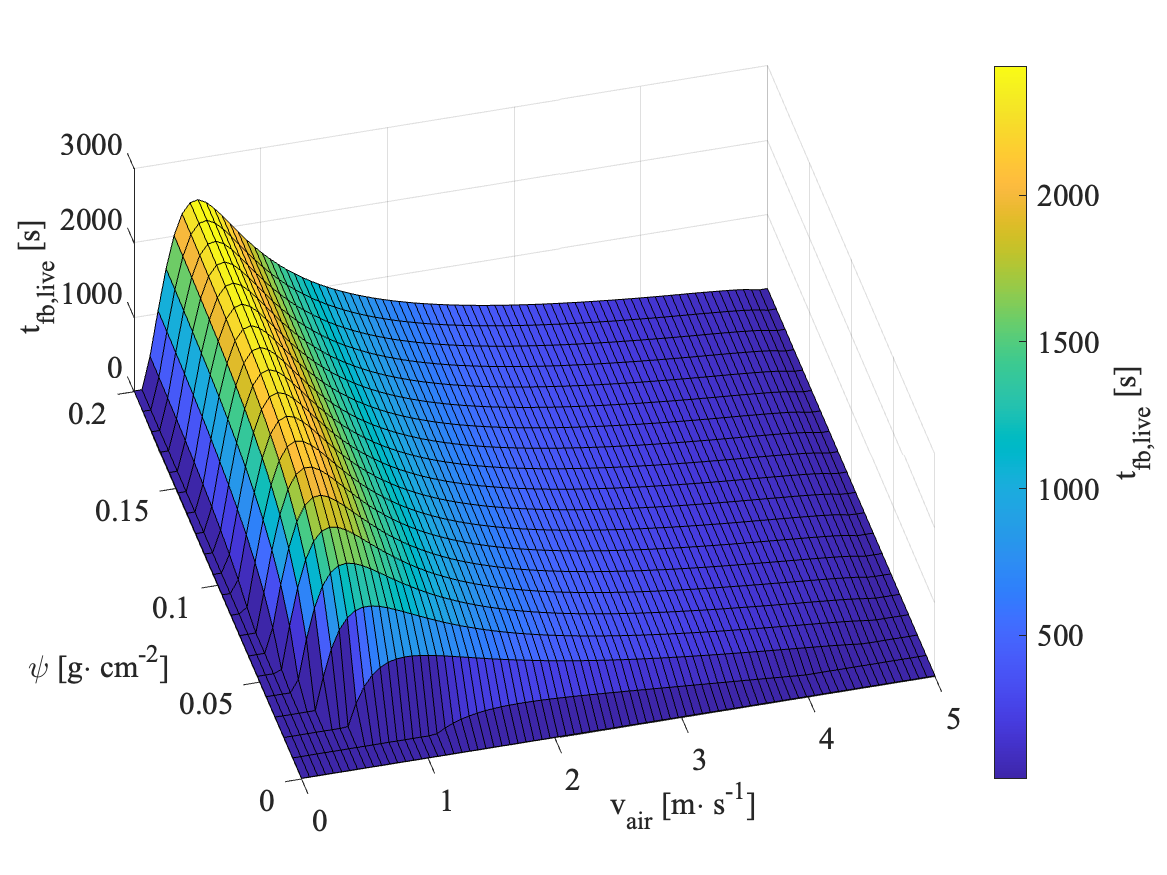
\includegraphics[width=4in]{./figs/fig_tactive_psi_vair.pdf}
%\renewcommand{\baselinestretch}{1}
%\small\normalsize
\captionsetup{margin={0in,0in}}
\caption{Predicted firebrand lifetime $t_{\text{fb,live}}$ as a function of ambient air velocity and local firebrand mass load $\psi$. ($HF_{\text{fb,live}} = 10~\mathrm{kW\cdot m^{-2}}$ and a minimum $t_{\text{fb,live}} = 10$~s are assumed)~\cite{qinPhysicsBasedEulerianFramework2025}.}
\label{fig:tactive_psi_vair}
\end{figure}
%\renewcommand{\baselinestretch}{2}
%\small\normalsize

To incorporate this formulation into ELMFIRE, a first-order explicit time integration scheme is applied, in which the local firebrand mass is updated simultaneously with the level-set variable $\phi$:

\begin{equation}
    \psi(t+\Delta t_l) = \psi(t) - \frac{\psi(t)}{t_{\text{fb,live}}\!\left(\psi(t),\, v_{\text{air}}(t)\right)} \, \Delta t_l.
\end{equation}

Here, $\Delta t_l$ denotes the time step used by the level-set equation solver.
\section{Smoke}

Estimating the smoke output of a specific wildfire scenario can be critical in assessing the health and visibility effects to nearby evacuees or to the wider populations through long term dispersion. To quantify the amount of smoke that people might be exposed to, a model is needed to estimate the dispersion of the wildfire pollutants (typically PM2.5) across the atmosphere. ELMFIRE does not contain such a model, but can prepare inputs for smoke dispersion models such as HYSPLIT. Models such as HYSPLIT require inputs relating to the amount of pollutants released by the wildfire, and the power of the plume convective column (which they use to estimate the rise height of the smoke plume). While the plume power can easily be inferred from the total heat release rate of the fire, quantifying the emissions of a wildfire is more challenging. 

The emissions of burning vegetation depend on a variety of factors, including the fuel loading, vegetation type, total consumption, fuel moisture content, and burning mode (flaming or smouldering). The information required for an accurate estimation of emissions is typically more than what fire behavior fuel types (Scott and Burgan, Andersen, NFDRS etc.) can provide. In the US, the FCCS fuel classification system was introduced to provide more information regarding the composition of a parcel of wildland \cite{ottmarOverviewFuelCharacteristic2007}. FCCS can be procured through the LANDFIRE database, similarly to fuel models, canopy information and digitised terrain data. This data can then be used in combination with emission estimation models such as FOFEM and FuelFireTools (through the coupling of FCCS model, CONSUME model and FEPS model). Each of these models can return an estimation of emissions per fuel stratum, burning mode, and the duration of each phase. 

Each of these models requires inputs from the user that would be difficult to obtain for theoretical fires. Parameters such as percent consumption of the canopy, percent sound and percent rotten wood are required by these models to provide accurate outputs. As such, and to ensure that ELMFIRE can be applied to global cases, a simplified method of estimating emissions has been implemented. 

Emission factors are experimental constants that relate the emission of specific products to the total consumed biomass. They can be found in the literature, estimated under lab conditions or from real burns. The values from \cite{reisenGroundBasedFieldMeasurements2018} are quoted below:

\begin{itemize}
    \item Flaming PM2.5: 17.4 $\pm$ 7.2 g/kg
    \item Smouldering PM2.5: 49.8 $\pm$ 32.1 g/kg
\end{itemize}

Note the significant error margins, reflecting the heterogeneity of actual emission factors depending on the local conditions and the burning vegetation. Compare these values with another source, providing literature review values of emission factors for US forests \cite{urbanskiWildlandFireEmissions2014}:

\begin{itemize}
    \item Flaming PM2.5 (Northwest conifer forests): 23.2 $\pm$ 10.4 g/kg
    \item Flaming PM2.5 (Boreal forests): 21.5 $\pm$ 4.8 g/kg
    \item Smoldering PM2.5 (Stumps and Logs) 33 $\pm$ 20 g/kg
    \item Smoldering PM2.5 (Temperate forest duff) 50 $\pm$ 16 g/kg
    \item Smoldering PM2.5 (Boreal forest duff) 20.6 $\pm$ 20.6 g/kg
\end{itemize}

The values are similar but show the difference between vegetation type and overall prevailing conditions. For ELMFIRE, the values of \cite{reisenGroundBasedFieldMeasurements2018} are used. The simplification is made that all fuel types (shrubs, grasses, timber litter etc.) have the same emission factors (and further down the section, calorific values). This simplification is maintained by anecdotal evidence that woody fuels produce the majority of PM2.5 emissions during a wildfire. 

The emission factors can be converted from grams per kilogram of burned biomass to grams per kiloJoule of emitted heat through the calorific value of wood. The net calorific value of wood depends strongly on the moisture content, as any water evaporation that occurs may drop the overall net heat release. Using the oven-dry wood calorific value, the following equation can be used:

\[
Q_{M}=Q_0(1-M)-2.44M
\]

With $Q_M$ being the net calorific value of wood with M\% moisture content, and $Q_0$ being the oven dry wood calorific value. According to literature, $Q_0$ is equal to 19 MJ/kg \cite{drysdaleIntroductionFireDynamics2011}.

For a specific pixel burning in the landscape, the total energy release during the flaming phase is:

\[
E=0.06\;I_b\;C^2\;R^{-1}
\]

With $E$ being the total energy release (MJ), $I_b$ being the fireline intensity (kW/m), C being the cell size (m), and R being the rate of spread (m/min). 

Thus for the flaming phase, the total emissions in a cell is equal to:

\[
PM_f = \frac{E\;\eta_f}{Q_M}
\]

With $\eta_f$ being the flaming emission factor. 

For smoldering combustion the above equation cannot be used, as the time scale for smouldering cannot be determined from a fireline intensity and rate of spread value. Smoldering is the more important burning mode during a wildfire with respects to harmful PM2.5 emissions, due to its incomplete combustion processes \cite{reinSmoulderingCombustionPhenomena2009}. The same source cites that more than 50\% of a forest's biomass can be burned during smoldering, depending on the ratios of the surface, canopy and ground fuel loading. In ELMFIRE, a more average value of 30\% is used, meaning that 70\% of the total burned biomass in a wildfire emits flaming-mode emissions and 30\% emits smodlering-mode emissions. Regarding the timespan of the smoldering phase of a wildfire, while no literature consensus exists, models like FOFEM predict values ranging from 30 to 60 minutes. 

Using the above, the smouldering emissions can be estimated through:

\[
PM_s = \frac{0.43E\;\eta_f}{Q_M}
\]

Typically, smoke outputs are saved hourly. While the flaming phase lasts about 5 minutes within a 30 x 30 m cell, the smouldering phase can last up to 60 minutes. If the flaming and smouldering emissions are added instantaneously to the total wildfire emissions, any transient effects would be ignored and the overall emission output would be over- or underestimated. To account for this, a subgrid scale model can be used based on the work in \cite{kalogeropoulosGaussianDispersionModel2025}. There, the total emissions for every time step are adjusted depending on the relative fire progression within the cell. In ELMFIRE a similar subgrid scale model is introduced, made different because of the different way of estimating emissions. For simulation time $T$ and cell ignition time $T_i$, the burning time of each cell is $T_c=T-T_i$. Then the relative total emissions of each cell can be linearly interpolated based on the total flaming time ($T_f=C/R$), and the total smoldering time ($T_s=60$ min). 


\section{Suppression}
\label{suppression}

The suppression module of ELMFIRE is experimental and still under development.
It does not attempt to model individual firefighter actions at specific times or
places, but instead represents the aggregate effects of suppression on wildfire
containment and fire growth.

There are two parts to the suppression module of ELMFIRE. The first estimates
the probability of success of an initial containment attempt based on fire size
and fireline intensity. The second represents extended attack. Two alternative
formulations are available for extended attack: an Area-Growth-Based Containment
Model and a Spatially Explicit Suppression Model. The former estimates an
aggregate target containment percentage, whereas the latter represents
suppression directly on the evolving fire perimeter through direct and indirect
attack.

\subsection{Initial Attack}

The approach used here to quantify initial attack probability of containment is
based on the analysis of Hirsch et al.
\cite{hirschUsingExpertJudgment1998}, who leveraged expert judgment to quantify
initial attack effectiveness as a function of fire size and head-fire fireline
intensity, i.e., intensity at the main advancing fire front at the time of
initial attack commencement. The authors developed an expression for probability
of containment (POC) as a function of fire size ($A$) and fireline intensity
($I_b$):

\[
POC = \frac{E}{1 + E},
\]

where

\[
\ln E =
4.6835
- 0.7043A
- 0.00041I_b
- 0.000052\,AI_b.
\]

In the equations above, $A$ is in hectares and $I_b$ is in kW/m. Since trends
in probability of containment are not immediately apparent upon inspection of
the equation, probability of containment calculated from the equation is
tabulated in Fig.~\ref{fig:poc_table} as a function of fire size and head-fire
fireline intensity at the time of initial attack. Although the qualitative
trends are logical, i.e., containment probability increases with smaller fires,
lower intensity, or both, the Hirsch et al. study was based on expert opinion
from Canadian firefighters, so differences in suppression tactics between
Canadian and U.S. agencies are not reflected in the formulation.

\begin{figure}[h]
    \centering
    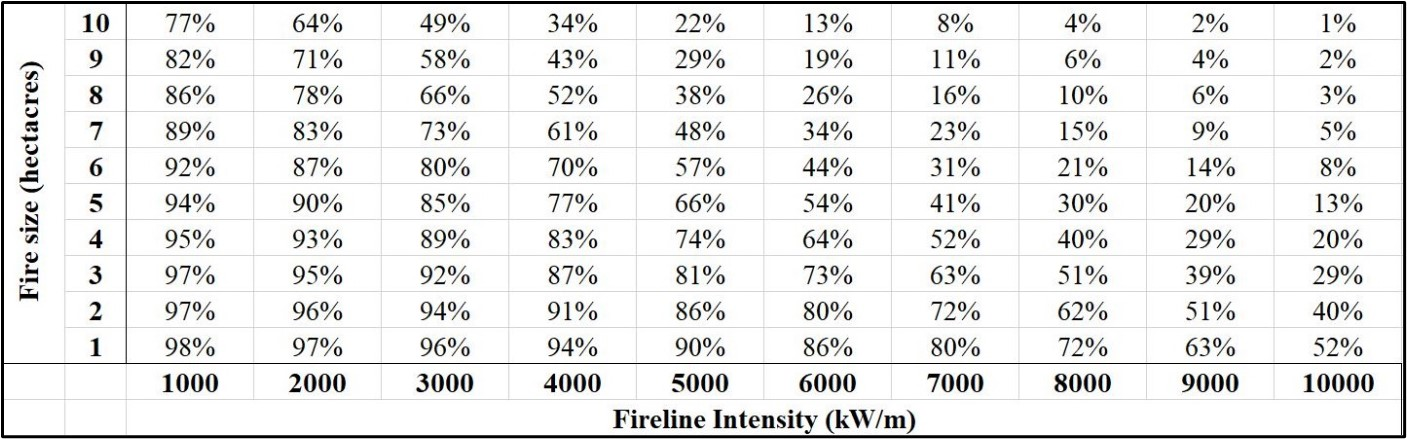
\includegraphics[width=1\linewidth]{figs/suppressionTable.png}
    \caption{Probability of successful initial attack calculated using the
    probability-of-containment formulation.}
    \label{fig:poc_table}
\end{figure}


\subsection{Extended Attack}

Extended attack in ELMFIRE can be represented using two alternative formulations.
The Area-Growth-Based Containment Model estimates a target containment fraction
from fire growth and suppression difficulty and subsequently distributes
containment around the fire perimeter. The Spatially Explicit Suppression Model
instead evaluates suppression directly on the evolving fireline and represents
direct attack and indirect control-location holding dynamically during fire
propagation.


\subsubsection{Area-Growth-Based Containment Model}

The aim of the Area-Growth-Based Containment Model is to estimate the target
containment of the fire at each suppression time step and compare it with the
estimated actual containment. It was developed based on a series of expert
judgment exercises, with quantification of containment per day depending on the
total containment capacity and daily progression of the fire.

At any given time step $t$ during the level-set fire-spread calculation, the
change in burning area can be calculated as

\[
\frac{\delta A}{\delta t}
=
\frac{A_t-A_{t-1}}{\Delta t}.
\]

For this equation and the remainder of this subsection,
$\delta A/\delta t$ is expressed in acres per day.

A critical parameter of extended suppression is the Suppression Difficulty
Index (SDI), a measure of the cumulative suppression difficulty of an area,
including the influence of factors such as terrain and accessibility. Based on
this value, total suppression difficulty can be represented through the
SDI-informed total fire acreage, calculated as the sum of all burning points on
the landscape multiplied by their corresponding SDI values:

\[
A_{SDI}
=
\sum_i A_i SDI_i.
\]

The change in cumulative suppression difficulty can then be calculated as

\[
\frac{\delta A_{SDI}}{\delta t}
=
\frac{A_{SDI,t}-A_{SDI,t-1}}{\Delta t}.
\]

The mean SDI at each time is subsequently calculated as

\[
\overline{SDI}_t
=
\frac{\delta A_T/\delta T}
     {\delta A_{SDI,T}/\delta T}
-1.
\]

The $\delta T$ terms are expressed in acres per day.
$\overline{SDI}_t$ is constrained to values between 0 and 3.

From this value, the change in target containment per day can be estimated based
on expert judgment as

\[
\delta C_{T,t}
=
0.01\psi C_m J
\exp\left(
-\left|B_{SDI}\overline{SDI}_t\right|
\right),
\]

where $\psi$ is the diurnal adjustment factor, $C_m$ is the maximum containment
per day, $B_{SDI}$ is a calibration constant, and $J$ represents the influence
of fire-area growth. The latter can be represented by either a linear or
logarithmic relationship:

\[
J
=
1-
\frac{\delta A/\delta t}{A_{nc}},
\]

or

\[
J
=
1-
\frac{\log(\delta A/\delta t)}
     {\log(A_{nc})},
\]

where $A_{nc}$ is the area-growth rate associated with no containment change
per day. In broad terms, the change in containment is primarily controlled by
the rate of fire-area increase relative to the specified area-growth threshold.

The total target containment at the current time step is then calculated as

\[
C_{T,t}
=
C_{T,t-1}
+
\delta C_{T,t}.
\]

The target containment is subsequently compared with the predicted actual
containment of the fire. The analysis evaluates cumulative containment by
dividing the fire front into angular bins relative to the centroid of the
burning area.

For a given angular bin $i$, the velocities of all points within the bin form
the set $V_i$, and the total number of cells within that bin is $N_i$. The
average velocity is therefore

\[
\overline{V}_i
=
\frac{\sum V_i}{N_i}.
\]

The suppressed fraction $s_i$ represents the fraction of previously suppressed
points within angular bin $i$.

The current containment before newly burning points are considered is estimated
as

\[
C_{C,p}
=
\sum_i s_i\frac{N_i}{N},
\]

where $N$ is the total number of burning or contained points over all angular
bins.

An intermediate step smooths the fire-front velocities by averaging the
velocities of neighboring angular bins. The effect of newly burning points is
then included until the current containment reaches the target containment:

\[
C_C
=
C_{C,p}
+
\sum_i
(1-s_i)\frac{N_i}{N}.
\]


\subsubsection{Spatially Explicit Suppression Model}

The Spatially Explicit Suppression Model represents suppression directly on the
evolving fire perimeter. Rather than prescribing a target containment percentage
for the entire fire, suppression develops through interactions between local
fire behavior, suppression difficulty, available suppression capacity, and
favorable control locations.

The model consists of two linked components. Direct attack represents
suppression conducted at or immediately adjacent to the active fire edge,
whereas indirect attack represents suppression opportunities at favorable
control locations ahead of the advancing fire. The resulting suppressed
portions of the fireline affect subsequent fire propagation.


\paragraph{Suppression Capacity and Deployment:}

Suppression capability is represented by the available suppression capacity,
$C_s(t)$, expressed as the length of fireline that can be treated per unit time.
The maximum available capacity is denoted by $C_{s,\max}$.

The model accounts for the delay associated with mobilization and deployment of
suppression resources. A fixed deployment time, $T_d$, can first be prescribed.
Under this formulation,

\[
C_s(t)
=
\begin{cases}
0, & t<T_d, \\[4pt]
C_{s,\max}, & t\geq T_d.
\end{cases}
\]

Thus, no extended-attack capacity is available before the prescribed deployment
time, after which the full suppression capacity becomes available.

Alternatively, the deployment time can be estimated from the early development
of the active fireline. Let $L(t)$ denote the active fireline length. The mean
fireline-growth rate during the first day of the simulation is estimated as

\[
\overline{G}_L
=
\frac{1}{N}
\sum_{k=1}^{N}
\frac{L(t_k)-L(t_{k-1})}
     {t_k-t_{k-1}},
\]

where $N$ is the number of fireline-growth intervals evaluated during the first
day.

A reference fireline length, $L_{\mathrm{ref}}$, represents the expected
fireline size at which full suppression capacity is deployed. The corresponding
deployment time is estimated as

\[
T_d
=
\frac{L_{\mathrm{ref}}}
     {\overline{G}_L}.
\]

For this approach, suppression capacity increases progressively from zero toward
the maximum available capacity during the deployment period. This relationship
can be expressed generally as

\[
C_s(t)
=
C_{s,\max}
f_{\kappa}
\left(
\frac{t}{T_d}
\right),
\qquad
0 \leq t<T_d,
\]

where

\[
f_{\kappa}(0)=0,
\qquad
f_{\kappa}(1)=1.
\]

Once the deployment time is reached,

\[
C_s(t)=C_{s,\max},
\qquad
t\geq T_d.
\]

The parameter $\kappa$ controls the shape of the capacity-development curve.
Larger values delay a greater fraction of the available capacity until later
in the deployment period and produce a sharper increase as the full-capacity
time is approached.


\paragraph{Direct Attack:}

Direct attack begins by identifying active fireline cells. An active fireline
cell is a burning cell adjacent to one or more unburned cells and therefore
represents a portion of the perimeter capable of continued propagation.
Isolated fireline cells are excluded to reduce grid-scale artifacts.

Each active fireline cell is classified according to fireline type as heading,
flanking, or backing fire. The classification follows the Huygens fire-spread
representation. A local fire-spread ellipse is associated with each active
fireline location, with its orientation and geometry determined by the combined
effects of wind, slope, aspect, and rate of spread. The position of the fireline
cell relative to the ellipse is then used to distinguish heading, flanking, and
backing portions of the fire.

The active fireline is subsequently divided into spatially connected segments
having similar fire behavior and suppression conditions. For neighboring cells
$j$ and $k$, similarity is evaluated using fireline type, rate of spread
($ROS$), flame length ($FL$), SDI, and PCL. The continuous-variable criteria can
be written as

\[
|ROS_j-ROS_k|
\leq
\Delta ROS,
\]

\[
|FL_j-FL_k|
\leq
\Delta FL,
\]

\[
|SDI_j-SDI_k|
\leq
\Delta SDI,
\]

and

\[
|PCL_j-PCL_k|
\leq
\Delta PCL.
\]

Very small segments are subsequently absorbed into neighboring segments to
reduce fragmentation and avoid highly irregular suppression patterns.

For each resulting segment $i$, the mean flame length and SDI are

\[
\overline{FL}_i
=
\frac{1}{N_i}
\sum_{j=1}^{N_i}FL_{ij},
\]

and

\[
\overline{SDI}_i
=
\frac{1}{N_i}
\sum_{j=1}^{N_i}SDI_{ij},
\]

where $N_i$ is the number of cells in segment $i$.

These quantities are normalized as

\[
FL_{n,i}
=
\frac{\overline{FL}_i}
     {FL_{\max}},
\]

and

\[
SDI_{n,i}
=
\frac{\overline{SDI}_i}
     {SDI_{\max}},
\]

where $FL_{\max}$ and $SDI_{\max}$ are reference values representing practical
limits for direct attack.

The relative feasibility and difficulty of direct attack are represented using
the Suppression Type Score ($STS$):

\[
STS_i
=
0.7FL_{n,i}
+
0.3SDI_{n,i}.
\]

The larger weighting assigned to flame length emphasizes the current fire
behavior at the active perimeter, while the SDI term accounts for additional
landscape-related suppression difficulty.

A fireline segment is considered eligible for direct attack when

\[
STS_i < 1.
\]

Segments satisfying

\[
STS_i \geq 1
\]

are not considered suitable for direct attack. Among eligible segments,
$STS_i$ also provides a relative measure of difficulty. Values approaching zero
represent favorable suppression conditions, whereas values approaching one
represent increasingly difficult conditions. Eligible segments are therefore
prioritized from the lowest to the highest $STS_i$.

Suppression difficulty also modifies the amount of capacity required to treat a
segment. Let $L_i$ denote the physical length of segment $i$. The effective
suppression requirement is calculated as

\[
L_{\mathrm{req},i}
=
\frac{L_i}
     {1-STS_i}.
\]

For relatively favorable conditions,

\[
STS_i \rightarrow 0
\quad\Longrightarrow\quad
L_{\mathrm{req},i}\rightarrow L_i.
\]

As suppression conditions become increasingly difficult,

\[
STS_i \rightarrow 1
\quad\Longrightarrow\quad
L_{\mathrm{req},i}\rightarrow\infty.
\]

The formulation therefore causes difficult segments to consume a larger portion
of the available suppression capacity than equal-length segments under more
favorable conditions.

For a suppression interval $\Delta t_s$, the total length that can be treated is

\[
L_{\mathrm{avail}}
=
C_s(t)\Delta t_s,
\]

when time and suppression-capacity units are consistent. If suppression capacity
is expressed in m/hr and the suppression interval is expressed in seconds, this
becomes

\[
L_{\mathrm{avail}}
=
C_s(t)
\frac{\Delta t_s}{3600}.
\]

Suppression is progressively applied to eligible segments until the available
capacity for the current suppression interval is exhausted.

Ranking segments only by $STS_i$ could cause suppression to alternate between
widely separated portions of the fire perimeter. The model therefore combines
the $STS_i$ ranking with a spatial search around the initial suppressed segment.
After the first segment is selected, subsequent attack locations are identified
through a $360^{\circ}$ angular search around the existing suppression location,
with preference given to nearby eligible segments having relatively low
$STS_i$. This allows suppression to progress more continuously along the active
fireline.


\paragraph{Indirect Attack:}

Indirect attack represents suppression at favorable control locations situated
ahead of the active fire edge. Potential Control Location (PCL) information is
used to identify areas where the advancing fire may be more likely to be stopped.

A cell $j$ is considered a candidate control location when

\[
PCL_j
\geq
PCL_{\mathrm{th}},
\]

where $PCL_{\mathrm{th}}$ is the minimum PCL value required for inclusion in the
candidate control network.

Spatially connected candidate cells are grouped into control-location segments.
The representative PCL value of segment $i$ is calculated as the mean PCL of
its constituent cells:

\[
\overline{PCL}_i
=
\frac{1}{N_i}
\sum_{j=1}^{N_i}
PCL_{ij},
\]

where $N_i$ is the number of cells belonging to control-location segment $i$.

For PCL represented on a scale from 0 to 100, the normalized control-location
suitability is

\[
PCL_{n,i}
=
\frac{\overline{PCL}_i}{100}.
\]

The probability that a control location successfully holds also depends on the
fire behavior present when the advancing fire encounters that location. Flame
length is used to represent this effect. The flame-length adjustment factor is

\[
F_{FL}
=
\frac{1}
     {1+\dfrac{FL}{FL_{\max}}},
\]

where $FL$ is the local flame length at the time of encounter and $FL_{\max}$ is
the same flame-length reference used in the direct-attack formulation.

For low flame lengths,

\[
F_{FL} \rightarrow 1,
\]

whereas increasing flame length progressively reduces $F_{FL}$. The formulation
therefore decreases the effectiveness of a potential control location as local
fire behavior becomes more severe.

The probability that control-location segment $i$ successfully holds is

\[
P_{\mathrm{hold},i}
=
PCL_{n,i}F_{FL}.
\]

The corresponding probability that the control location is breached is

\[
P_{\mathrm{breach},i}
=
1-P_{\mathrm{hold},i}.
\]

When the advancing fire reaches a candidate control location, the outcome is
determined stochastically. A random value $R$ is drawn from a uniform
distribution,

\[
R
\sim
U(0,1).
\]

The control location successfully holds when

\[
R
\leq
P_{\mathrm{hold},i}.
\]

In this case, propagation through the affected portion of the control location
is prevented. Conversely, if

\[
R
>
P_{\mathrm{hold},i},
\]

the control location is considered breached and the fire continues to propagate
according to the underlying ELMFIRE fire-spread calculation.





















\section{Urban Fire Spread}

The urban fire spread model adapted in ELMFIRE is WU-E, taken from Purnomo et al \cite{purnomoReconstructingModesDestruction2024}, and describes a semi-physical model to estimate the spread of fire though a built-up area, which up to now was considered nonburnable by Rothermel-based fire models. 

The heat transfer from a fire front to a nearby building is broken down into direct flame contact (DFC), radiation and firebrands. Each of the three heat transfer mechanisms is assumed independent, although areas with direct flame contact do not calculate radiation as well. The heat transfer mechanisms considered here are shown in Fig. \ref{fig:wueheatspread}.

\begin{figure}
    \centering
    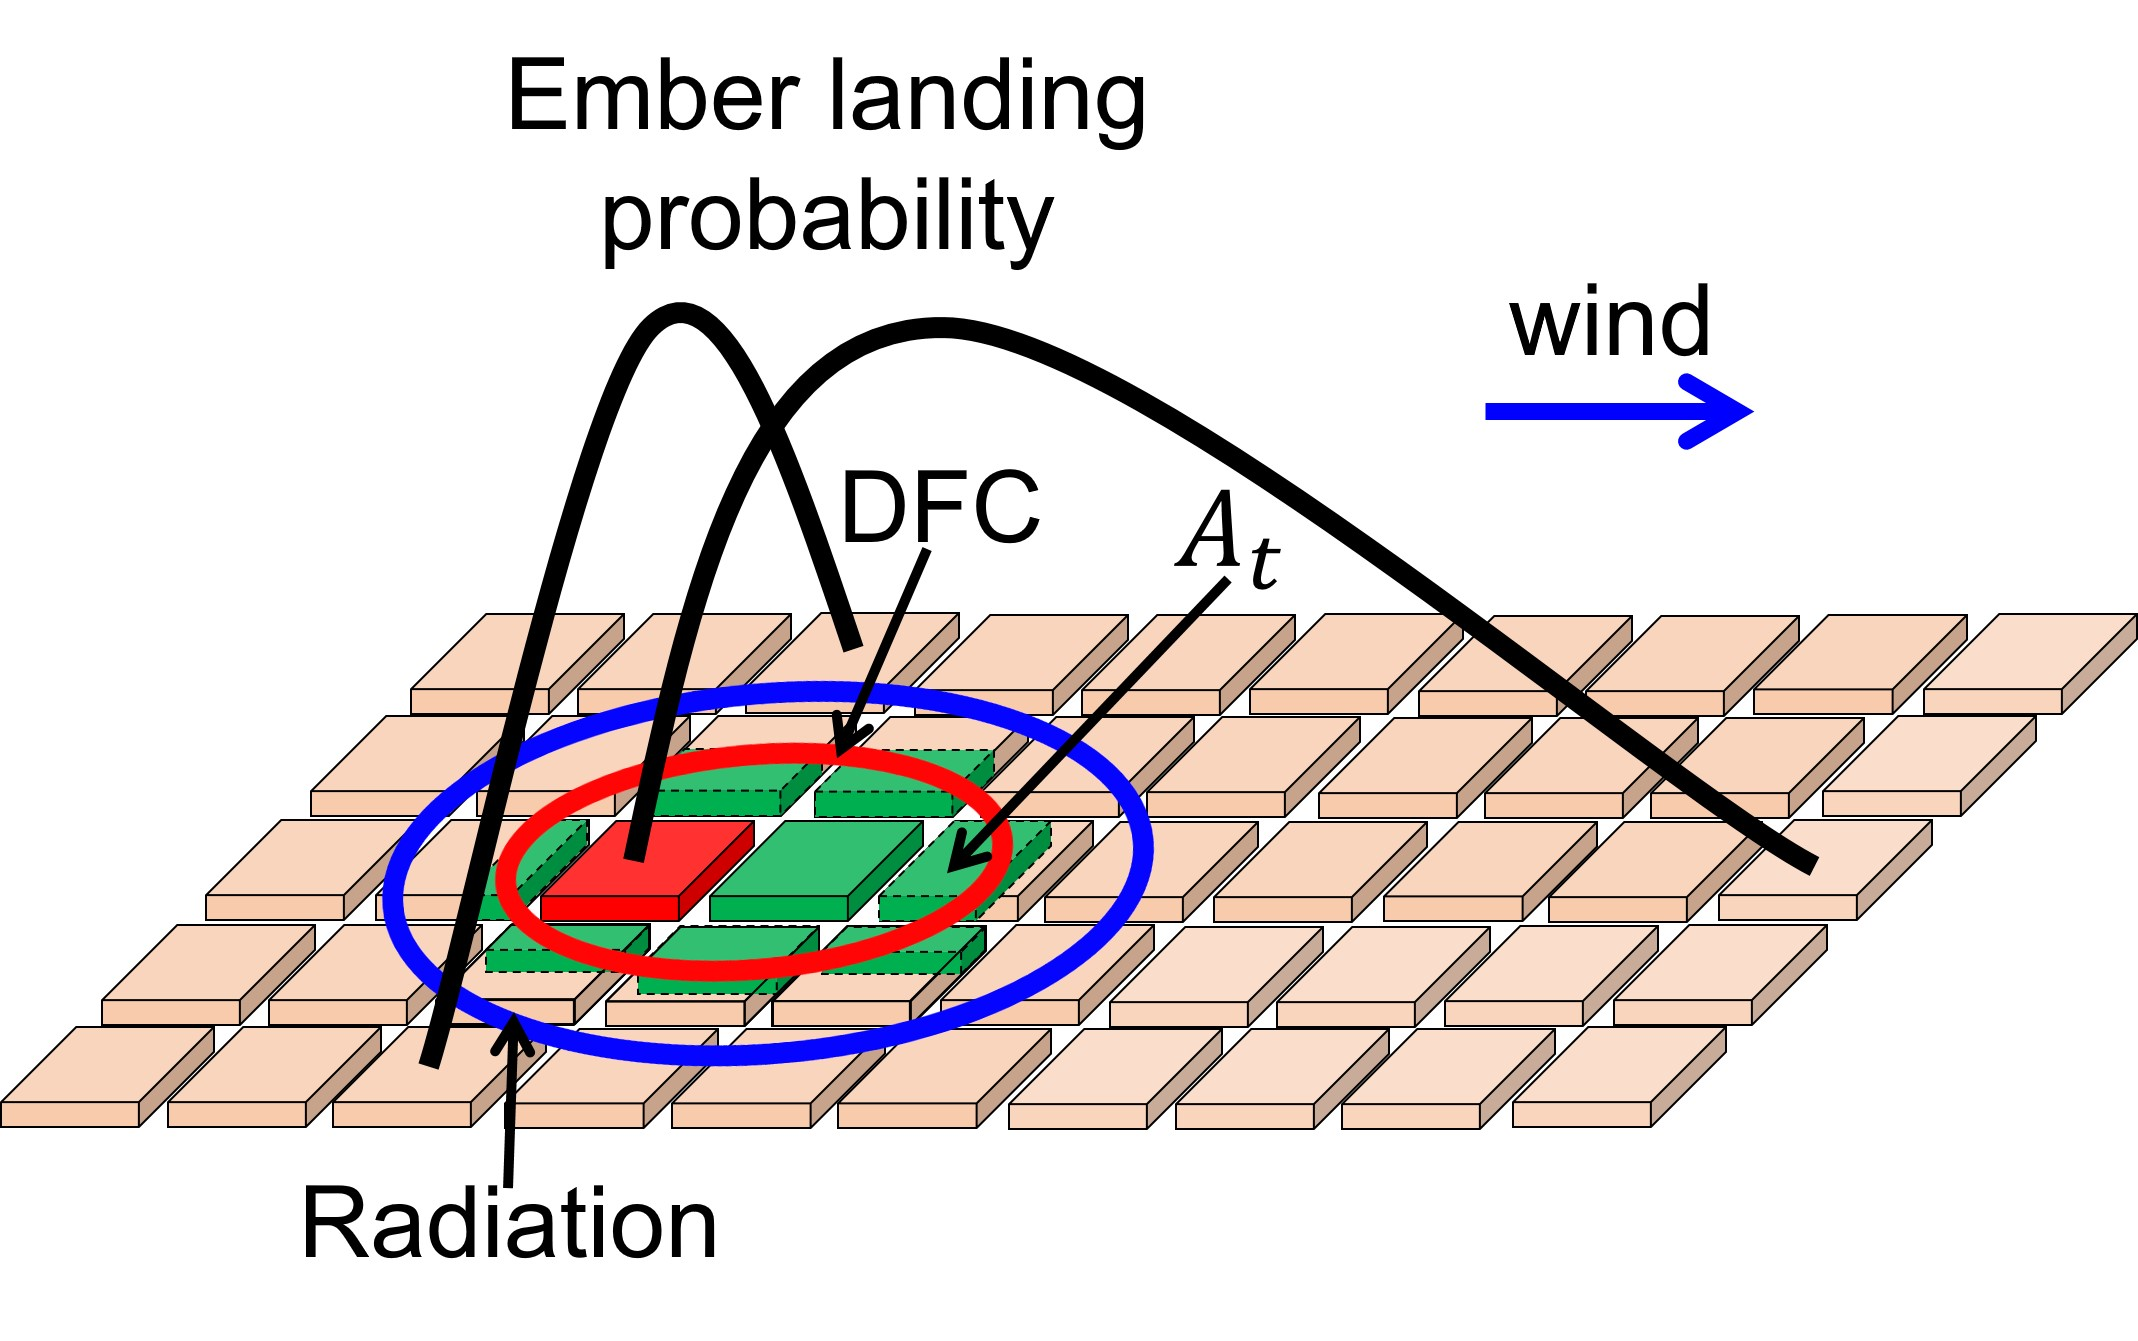
\includegraphics[width=0.5\linewidth]{figs/wuefireTransfer.jpg}
    \caption{A schematic of the WU-E heat spread mechanisms}
    \label{fig:wueheatspread}
\end{figure}

The model operates by simulating multiple modes of fire spread. Heat transfer to cells via DFC is determined by the heat release rate (HRR) and the relative position of the target cell to the burning structure. Currently, this component of the model is based on regression data from the older Hamada model \cite{hamadaRateFireSpread1951}, as fine-scale data for structure-to-structure heat fluxes remains limited. For direct flame contact, the Hamada model \cite{hamadaRateFireSpread1951} is used to estimate its range of effect. Due to the rarity of digital copies of this work, the Hamada model as explained by Qin \cite{qinPhysicsBasedEulerianFramework2025} has been repeated below.

For radiative heat transfer, the model employs a point-source ignition approach to account for radiation effects. Consequently, fire spread via radiation is also influenced by HRR. Structures ignite when they are exposed to a critical heat flux for a specified duration, defined as a flux-time product, which represents the ignition characteristics of the material.



\subsection{The Hamada Model}

The Hamada model was developed for a point source building ignition, in a uniform community. It calculates the fire spreads based on an elliptical assumption, explicitly calculating the spread of the fire downwind ($K_d$), upwind ($K_u$), and crosswind ($K_s$). These parameters are enough to get a Length over Width (LoW) measure, that can be directly applied using the elliptical fire spread equations we have already established. 

The original elliptical dimensions are: 

\[
K_d = \frac{(a_0 + d)\,t}{T_d},
\]

\[
K_s = \frac{a_0}{2} + d + \frac{(a_0 + d)(t - T_s)}{T_s},
\]

\[
K_u = \frac{a_0}{2} + d + \frac{(a_0 + d)(t - T_u)}{T_u}.
\]

With $a_0$ denoting average building footprint dimension, $d$ is average building separation, and $t$ is the elapsed time. A later correction by Hazus was introduced to correct for an overestimation of fire spread under zero wind:

\[
K'_{d}
= K_{d}\frac{V}{10}
+ \left(1 - \frac{V}{10}\right)
  \sqrt{\left(\frac{K_{d} + K_{u}}{2}\right)}\,K_{s},
\]

\[
K'_{s}
= K_{s}\frac{V}{10}
+ \left(1 - \frac{V}{10}\right)
  \sqrt{\left(\frac{K_{d} + K_{u}}{2}\right)}\,K_{s},
\]

\[
K'_{u}
= K_{u}\frac{V}{10}
+ \left(1 - \frac{V}{10}\right)
  \sqrt{\left(\frac{K_{d} + K_{u}}{2}\right)}\,K_{s}.
\]

Where $V$ is the wind speed. The above equations can be rearranged to solve for the time taken for the fire to reach adjacent buildings. 

\[
T_i
=
(1 - f_b)\left(
  3 + 0.375\,a_0
  + \frac{8d}{\,c_{4i} + c_{5i}V\,}
\right)
+
\frac{f_b}{C(V)}\left(
  5 + 0.625\,a_0
  + \frac{16d}{\,c_{4i} + c_{5i}V\,}
\right),
\]

\[
C(V) = c_{1i}\bigl(1 + c_{2i}V + c_{4i}V^{2}\bigr).
\]


where $i$ indexes wind directions (downwind, crosswind, upwind), and $f_b$ is the combustible fraction. Empirical constants $c_{ki}$ are tabulated below:

\begin{table}[h!]
\centering
\begin{tabular}{c c c c c c}
\hline
$i$ & $c_{1i}$ & $c_{2i}$ & $c_{3i}$ & $c_{4i}$ & $c_{5i}$ \\
\hline
d & 1.6 & 0.1 & 0.007 & 25.0 & 2.5 \\
s & 1.0 & 0.0 & 0.005 & 5.0  & 0.25 \\
u & 1.0 & 0.0 & 0.002 & 5.0  & 0.2 \\
\hline
\end{tabular}
\end{table}

Then, the spread extent and spread time can be used to find the rate of spread of the fire towards each direction:
\[
V_i
= \frac{dK'_i}{dt}
= \frac{V}{10}\,\frac{dK_i}{dt}
+ \frac{1}{4}\left(1 - \frac{V}{10}\right)\mathcal{A},
\qquad i \in \{d,s,u\}.
\]


\[
\mathcal{A} :=
\sqrt{\frac{2}{(K_d + K_u)\,K_s}}
\left[
  \frac{dK_s}{dt}(K_d + K_u)
  + K_s\!\left(\frac{dK_d}{dt} + \frac{dK_u}{dt}\right)
\right].
\]

With the temporal derivatives:

\[
\frac{dK_i}{dt}=\frac{a_0+d}{T_i}
\]

The results can then be used to calculate the LoB of the urban fire spread ellipse:

\[
LB = \frac{V_u+V_d}{V_s}
\]

\subsection{Heat Transfer}

DFC, originating from a burning house (red square), has limited influence, depicted by the red ellipse. Beyond this ellipse, DFC is negligible. Radiation effects are confined to a 100-m radius (blue ellipse) and are zero beyond this distance. When a cell receives DFC, only heat from DFC is considered, disabling radiation. For cells with both DFC and radiation, heat contributions are shown by green (DFC) and brown (radiation) areas. Firebrand propagation follows probabilistic distributions.

The heat transferred to cells via DFC is determined by the heat release rate (HRR) and the relative position of the cell to the burning house. This relationship is formulated as:

\[\dot{q}_c = \frac{HRR \cdot A_t}{A_{f,eff}}\]

Here, $\dot{q}_c (kW)$ is the heat from DFC, $HRR$ (kW) is the heat release rate of a source cell, $A_t (m^2)$ is the area of a target cell affected by the flame, and $A_{f,eff}(m^2)$ is the effective flame area. The flame size is determined by regression based on Hamada's empirical model, considering wind speed, house size, and separation distance.

The HRR starts at zero upon ignition, grows linearly to peak HRR, stays constant, and then decays as fuel is consumed. Peak HRR per unit area of structure (HRRPUA) is 150 $kW/m^2$, calculated by dividing the reported HRR by the structure area. Stages include an early stage (5 min), a fully developed stage (1 min), and a decay stage (60 min).

The model adopts a point-source ignition method for radiation effects. The spread of fire through radiation depends on HRR and the distance of the target cell from the burning house. The incident heat flux resulting from radiation is calculated as:
\[
\dot{q}_r'' = \frac{0.3 \cdot HRR}{4\pi R^2}
\]

Fire spread from urban cells to neighboring cells depends on heat transfer via DFC, radiation, or firebrands. Heat received by an unburned cell is given by:

\[
\dot{q}_t = \alpha_c \dot{q}_c + \alpha_r \dot{q}_r'' \Delta x^2
\]

where $\alpha_c$ and $\alpha_r$ are fire transfer coefficients for DFC and radiation, and $\Delta x^2$ is the area of the burning house. The DFC coefficient $\alpha_c$ depends on house material and configuration, while the radiative coefficient $\alpha_r$ is a product of $\alpha_c$ and house radiation absorptivity. The DFC coefficient $\alpha_c$ is derived from:

\[\alpha_c = \frac{S_b + S_v}{S_t}\]
where $S_b$ is the combustible material surface area, $S_v$ is the vegetation area outside the house within the same cell, and $S_t$ is the total surface area.

A structure ignites when subjected to a critical heat flux for a duration defined by the critical flux time product (FTP). The FTP value ($kJ$) is based on incident heat flux, adapted from Lee (2009). The model can account for different FTP values for various materials, though a uniform threshold is used here. The model’s flexibility allows easy integration of future improvements based on new research.

For urban fire spread rate, $U$ represents the time $\Delta t$ required to ignite a structure of size $\Delta x$, as shown by:

$\sum \left(\dot{q}_t\Delta t\right) \geq FTP$


$U = \frac{\sum \dot{q}_t}{FTP} \cdot \Delta x$

It can be expressed as a vector by applying decomposition through the elliptical point spread hypothesis:


\[
a = \frac{K_d + K_u}{2},
\]

\[
c = \min\!\left( \frac{a}{2},\, a - K_u \right),
\]

\[
b = \frac{K_s}{\sqrt{\,1 - \left(\tfrac{c}{a}\right)^{2}}}.
\]

And the directional rates of spread can be calculated downwind ($V_d$), upwind ($V_u$), and sidewind ($V_S$) of the source:

\[
V_d = U \cdot \frac{(a + c)\,\Delta x}{2(a + b)},
\]

\[
V_s = U \cdot \frac{2b\,\Delta x}{2(a + b)},
\]

\[
V_u = U \cdot \frac{(a - c)\,\Delta x}{2(a + b)}.
\]

The model also adapts for fire spread from vegetation into urban areas by converting the wildland fireline intensity output to HRR for modeling urban fire spread. However, a simplified version of this interface spread is introduced. This simplified version leverages distance from burning vegetation and fireline intensity threshold to determine ignition of structures caused by burning vegetation. The default values for these thresholds are now arbitrary selected as 1 cell for distance and 1000 kW/m for fireline intensity. These two interface spread options can be selected depending on the users and purposes.

Similarly, when fire spreads from urban to wildland areas, wildland cells at the urban interface receive heat from adjacent urban cells and ignite accordingly, using the same equations as for urban cells.

$HRR = I_f \Delta x$ 

A number of critical assumptions need to be taken into account when using this model.

\begin{itemize}
    \item The heat received by the target is the heat flux times the area affected (At). It is assumed that the heat flux is uniform over the flame ellipse. Thus, the heat flux is HRR/area. It is assumed that the heat flux when the heat flux gauge is placed on the wall of the burning house is equal to the heat flux gauge reading when place further away from the burning house as long as the flame touches the heat flux gauge.
    \item Regression is performed on Hamada equations, adapting the method in Jiang, so that WU-E does not execute Hamada equation, which can be more computationally demanding, but instead calculates the more simple regression equation. From these calculations, flame reach at the downwind, upwind and sidewind directions are obtained. These flame reaches cannot be directly used to get the radius of ellipse at a specific angle, that follow Kepler law of elliptical orbit.

    \item The ellipse area used for the calculation of DFC is based on effective ellipse area. Although the real flame ellipse might be larger, the heat dissipates more rapidly further from the source. By focusing on a smaller effective ellipse, where the majority of the heat is actually distributed, we assume uniform heat within this area and negligible heat outside it (but still within the real ellipse). This approach prioritizes the area closer to the source, effectively sacrificing the outer regions, formulated as:
    
    \[
    \dot{q}_c = \frac{HRR \cdot A_t}{\pi \cdot a_{\text{eff}} \cdot b_{\text{eff}}}
    \]
    
    To accommodate this, a tunable parameter (\texttt{HRR\_ELLIPSE\_ADJ}) was introduced in the SIMULATOR namelist. This parameter is multiplied with the actual semi-major and semi-minor axes of the ellipse to obtain their effective values used in the calculation. The default value of \texttt{HRR\_ELLIPSE\_ADJ} is set to 0.5, but it is subject to calibration for improved accuracy.
       
    \item C\%ABSOLUTE\_U corresponds to the total heat available to form the flame ellipse. It is assumed that by determining the portion of this heat goes to downwind (C\%VELOCITY\_DMS), upwind (C\%VBACK ), and sidewind (V\_S), ellipse shape can be formed. Thus, C\%ABSOLUTE\_U corresponds to the total of these portions (sum of downwind, upwind, and sidewind directions). The fraction of C\%ABSOLUTE\_U goes to downwind (C\%VELOCITY\_DMS), upwind (C\%VBACK ), and sidewind (V\_S) are based the ratio of each length with the total length.
\end{itemize}

\section{Diurnal Profiles}

The diurnal factors, aiming at adjusting for the Rothermel model's known overestimation of night-time rate of spread, require an estimation of the sunrise and sunset times of the area of interest. The calculations used in ELMFIRE come from the NOAAs sunrise/sunset calculations, and will be repeated here:

The fractional year $\gamma$, in radians, is computed as:
\[
\gamma =
\frac{2\pi}{365}
\left(
\mathrm{day\_of\_year} - 1
+
\frac{\mathrm{hour} - 12}{24}
\right)
\]
For leap years, replace 365 with 366.

Using $\gamma$, we compute the equation of time (in minutes):
\[
\mathrm{eqtime} = 229.18 \left(
0.000075
+ 0.001868\cos\gamma
- 0.032077\sin\gamma
- 0.014615\cos(2\gamma)
- 0.040849\sin(2\gamma)
\right)
\]

The solar declination angle (in radians) is:
\[
\mathrm{decl} =
0.006918
- 0.399912\cos\gamma
+ 0.070257\sin\gamma
- 0.006758\cos(2\gamma)
+ 0.000907\sin(2\gamma)
- 0.002697\cos(3\gamma)
+ 0.00148\sin(3\gamma)
\]

First compute the total time offset (minutes):
\[
\mathrm{time\_offset}
=
\mathrm{eqtime}
+ 4(\mathrm{longitude})
- 60(\mathrm{timezone})
\]
Longitude is in degrees, positive east of the prime meridian.  
Timezone is hours from UTC (e.g., U.S. Mountain Standard Time = $-7$).

Then the true solar time (minutes) is:
\[
\mathrm{tst} =
\mathrm{hr} \cdot 60
+ \mathrm{mn}
+ \frac{\mathrm{sc}}{60}
+ \mathrm{time\_offset}
\]

The solar hour angle (degrees) is:
\[
\mathrm{ha} = \frac{\mathrm{tst}}{4} - 180
\]

The solar zenith angle $\phi$ is given by:
\[
\cos\phi
=
\sin(\mathrm{lat}) \sin(\mathrm{decl})
+
\cos(\mathrm{lat}) \cos(\mathrm{decl}) \cos(\mathrm{ha})
\]

The solar azimuth angle $\theta$ (degrees clockwise from north) satisfies:
\[
\cos(180 - \theta)
=
-
\frac{
\sin(\mathrm{lat}) \cos\phi
-
\sin(\mathrm{decl})
}{
\cos(\mathrm{lat}) \sin\phi
}
\]

For sunrise or sunset, the zenith angle is set to:
\[
z_0 = 90.833^\circ
\]
accounting for atmospheric refraction and solar disk radius.

The corresponding hour angle is:
\[
\mathrm{ha}
=
\pm \arccos
\left\{
\frac{
\cos z_0
}{
\cos(\mathrm{lat}) \cos(\mathrm{decl})
}
-
\tan(\mathrm{lat}) \tan(\mathrm{decl})
\right\}
\]
The $+$ sign corresponds to sunrise, $-$ to sunset.

\[
\mathrm{sunrise}
=
720
-
4(\mathrm{longitude} + \mathrm{ha})
-
\mathrm{eqtime}
\]
(all angles in degrees, eqtime in minutes).

Solar noon occurs at:
\[
\mathrm{snoon} =
720 - 4(\mathrm{longitude}) - \mathrm{eqtime}
\]



